\newpage
\chapter{Разширени графични възможности и вероятностни разпределения}
\label{chapter08}
\thispagestyle{empty}

\section{Разширени графични възможности}

Към базовите графични възможности на R, пакетите $ggplot2$ и $lattice$ добавят множество допълнителни функционалности. Синтаксисът на извикванията леко се различава от този на функциите в базовите възможности, но това създава затруднения само в началния етап от употребата на двата пакета. 

За визуализация, чрез $ggplot2$ като основа се използва функцията $ggplot$. В общия случай тази функция получава, като входен параметър данните за визуализиране и понякога някои допълнителни параметри. Резултатът от изпълнението на $ggplot$ е обект, който в последствие може да бъде допълнително променян, чрез добавяне на възможности с помощта на операцията събиране (+). 

\subsection{Хистограми и плътности}

Хистограмата\index{хистограма} служи за групиране на стойностите и изброяване на това колко стойности попадат по определените групи. Размерът на всяка група (bin) определя ширината на стълба. 

\begin{lstlisting}[caption=Хистограма и плътност, label=listing0150]
library(ggplot2)

ggplot(data=diamonds) + geom_histogram(aes(x=carat))

ggplot(data=diamonds) + geom_density(aes(x=carat),fill="grey50")
\end{lstlisting}

Както и в предходния пример за хистограма, тук също е представено разпределението на диамантите по карати (Листинг \ref{listing0150}).

\begin{figure}[h!]
  \centering
  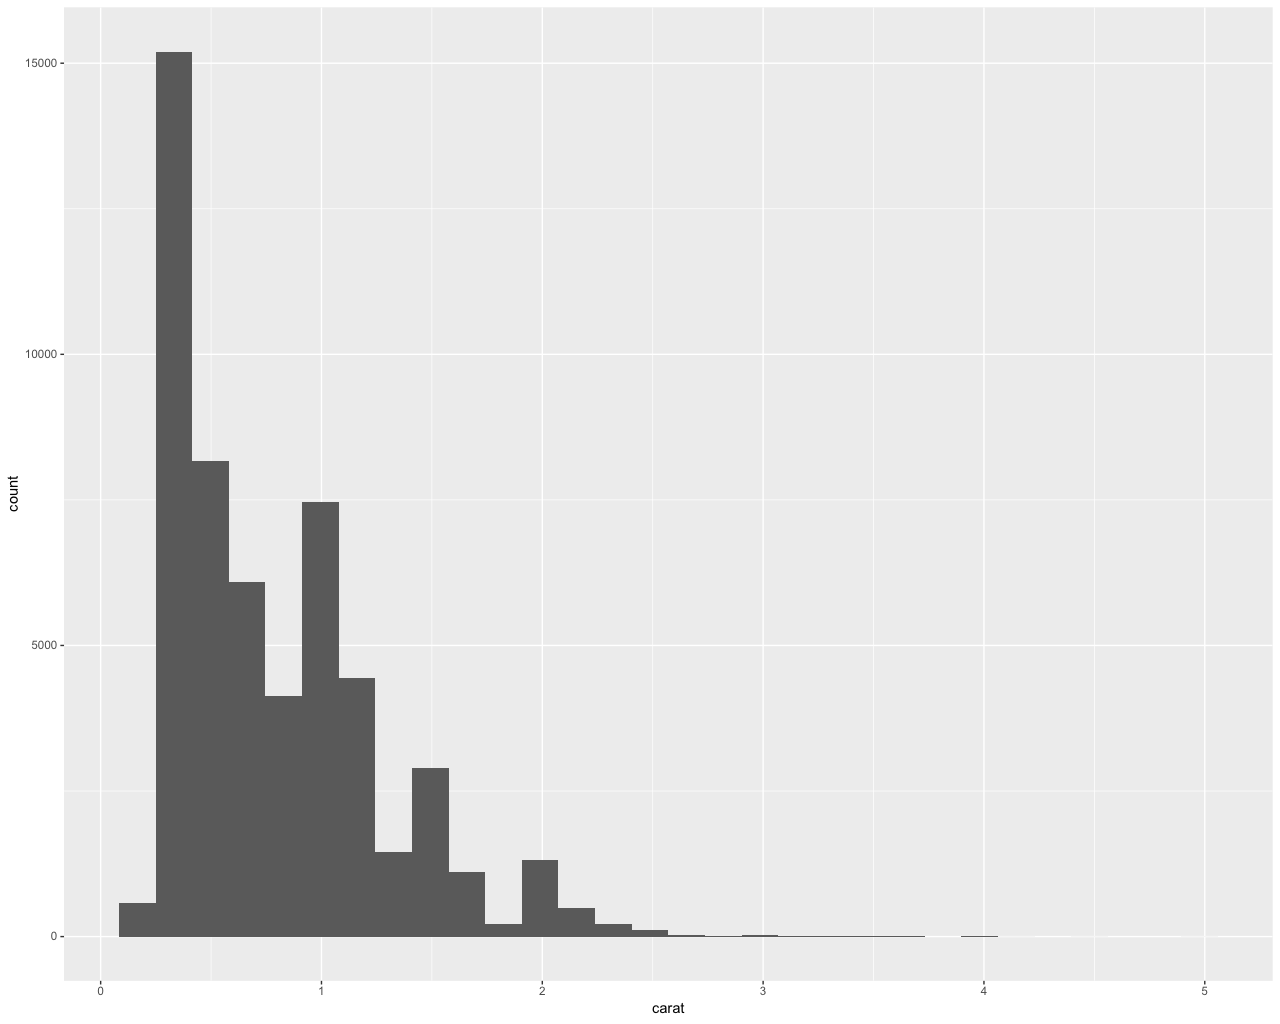
\includegraphics[width=1.0\linewidth]{pic0030}
  \caption{Хистограма при 30 групи}
\label{figure0030}
\end{figure}
\FloatBarrier

Функцията $aes$ определя кои данни да бъдат използвани за разполагане по осите. В примера с диамантите, това е характеристиката за тегло (карат). 

\begin{figure}[h!]
  \centering
  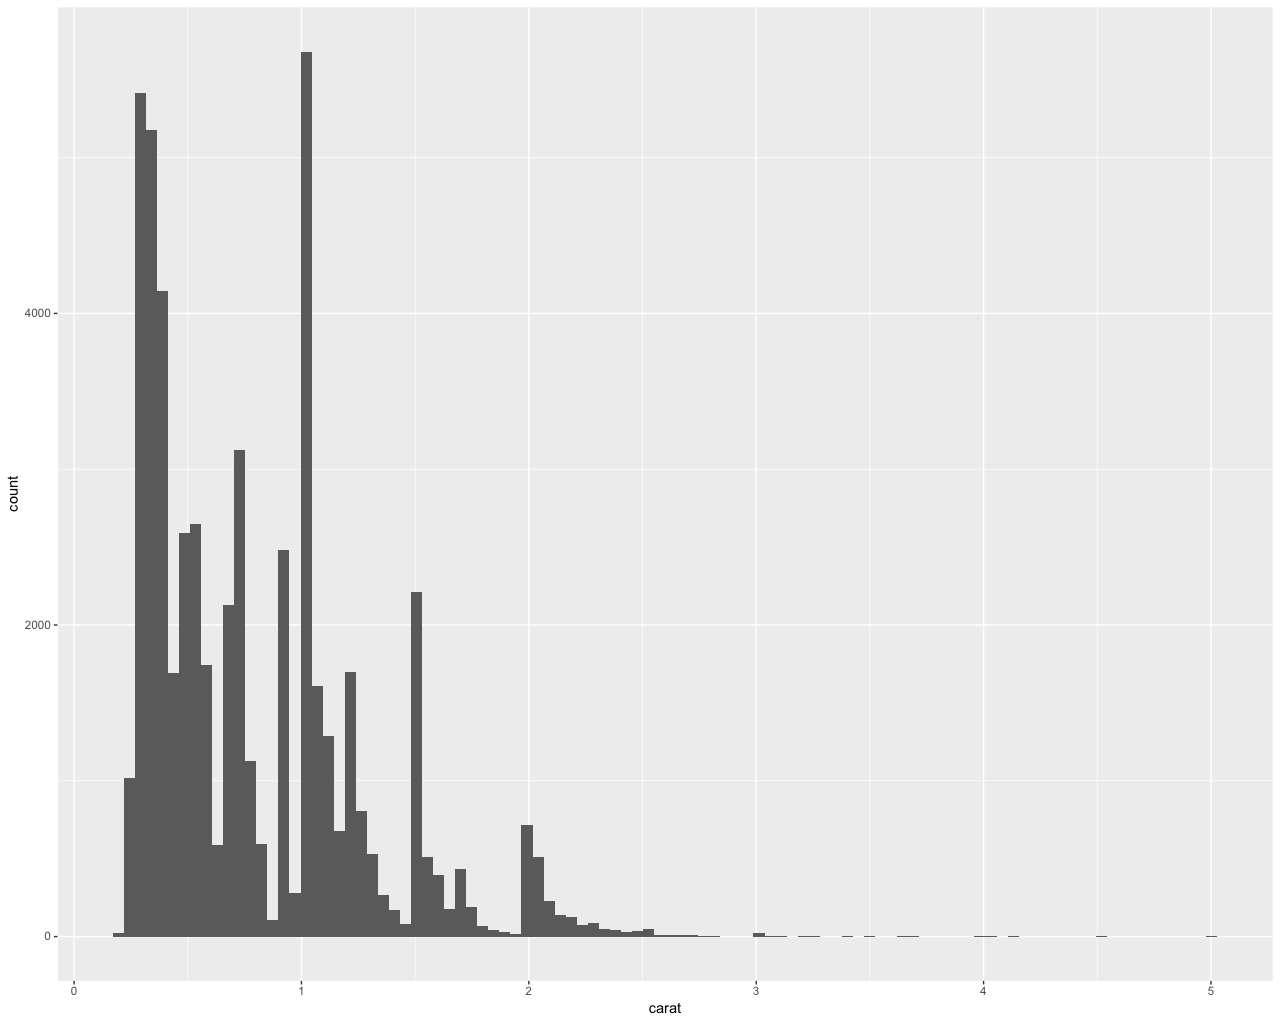
\includegraphics[width=1.0\linewidth]{pic0031}
  \caption{Хистограма при 100 групи}
\label{figure0031}
\end{figure}
\FloatBarrier

Размерът на групите в хистограмата може да варира (Фиг. \ref{figure0030},\ref{figure0031}). За да се изчертае плътностна функция\index{плътностна функция} е достатъчно графичният обект, генериран от $ggplot$, да бъде декориран с функцията $geom\_density$ (Фиг. \ref{figure0032}), вместо с функцията $geom\_histogram$. 


\begin{figure}[h!]
  \centering
  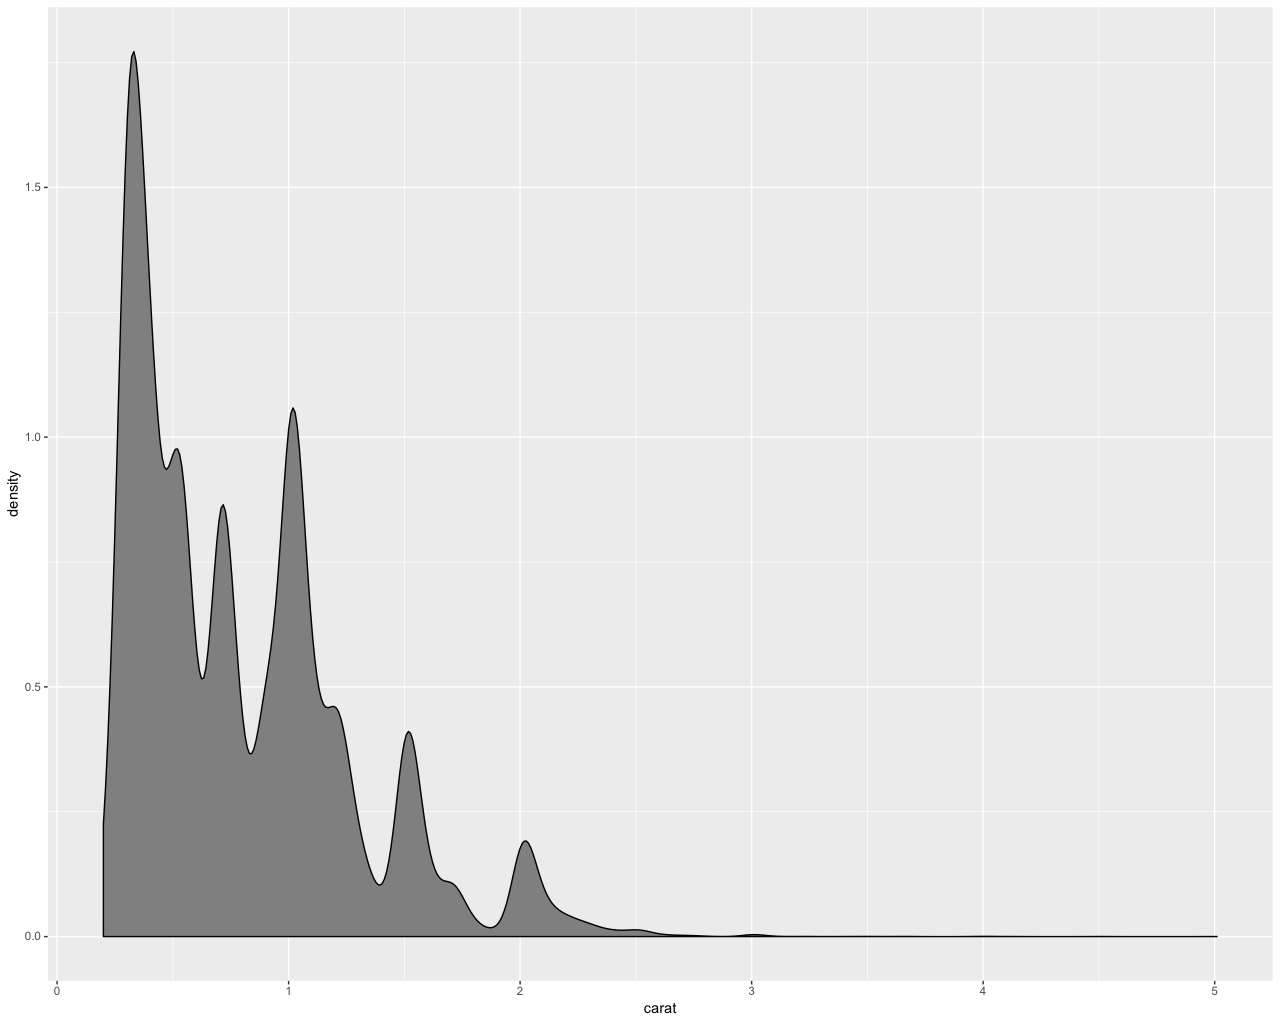
\includegraphics[width=1.0\linewidth]{pic0032}
  \caption{Плътностна функция}
\label{figure0032}
\end{figure}
\FloatBarrier

Хистограмата показва броене по групи, докато плътностната функция задава вероятността определен камък да попадне в предварително определен интервал. Макар и много да си приличат, хистограмата и плътностната функция са подходящи в два различни случая. Хистограмите са полезни при дискретни случайни величини, докато плътностните функции намират повече употреба в непрекъснатите случайни величини. 

\subsection{Диаграми на разсейване}

Пакетът $ggplot2$ разширява възможностите за визуализация на диаграми на разпръскване\index{диаграма на разпръскване}, които базовата функционалност на R предлага (Листинг \ref{listing0151}). 

\begin{lstlisting}[caption=Диаграма на разпръскване с ggplot2, label=listing0151]
library(ggplot2)
ggplot(diamonds, aes(x=carat, y=price)) + geom_point()
\end{lstlisting}

Функцията $aes$ определя кои колони от множеството данни да се използват при визуализацията (Фиг. \ref{figure0033}). Пакетът $ggplot2$ дава и друго много съществено предимство, графиката която ще се изчертава да бъде съхранена в отделен обект, на който обект след това да се добавят различни визуални декорации (обектът $c2p$ от примера).

\begin{figure}[h!]
  \centering
  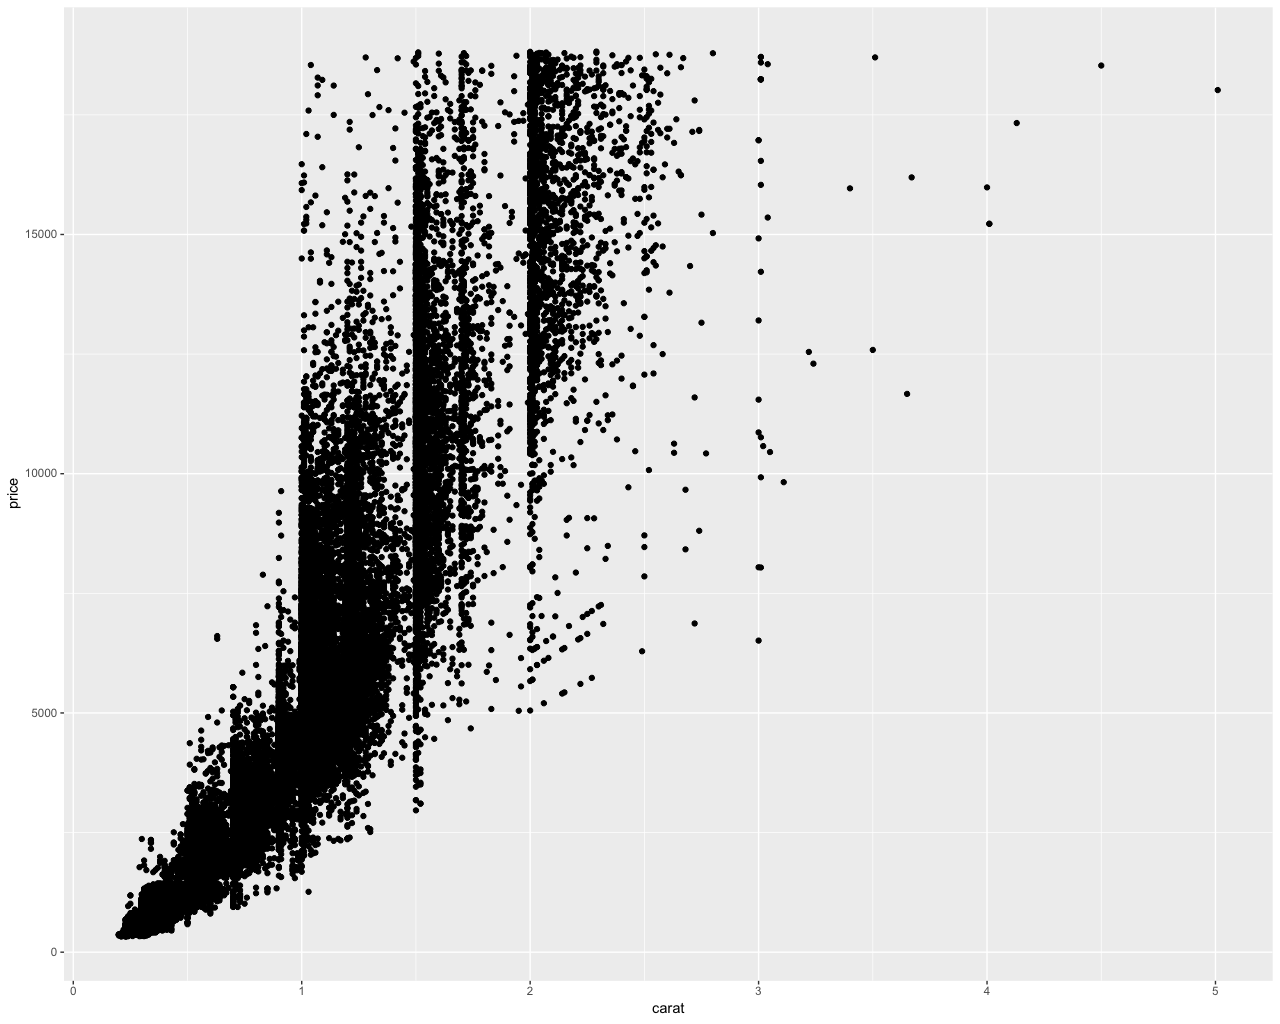
\includegraphics[width=1.0\linewidth]{pic0033}
  \caption{Диаграма на разпръскване с ggplot2}
\label{figure0033}
\end{figure}
\FloatBarrier

Пакетът дава възможности и за подреждането на група от диаграми на разсейването. Това се постига с някоя от функциите $facet\_wrap$ или $facet\_grid$ (Листинг \ref{listing0152}). 

\begin{lstlisting}[caption=Диаграма на разпръскване групирани по признак, label=listing0152]
c2p <- ggplot(diamonds, aes(x=carat, y=price))

c2p + geom_point(aes(color=color)) + facet_wrap(~color)

c2p + geom_point(aes(color=color)) + facet_grid(clarity~cut)
\end{lstlisting}

Функцията $facet\_wrap$ разделя множеството от данните на групи, според зададения признак (в примера това е цветът на диамантите) и след това формира диаграма на разпръскване за всяка от групите (Фиг. \ref{figure0034}).

\begin{figure}[h!]
  \centering
  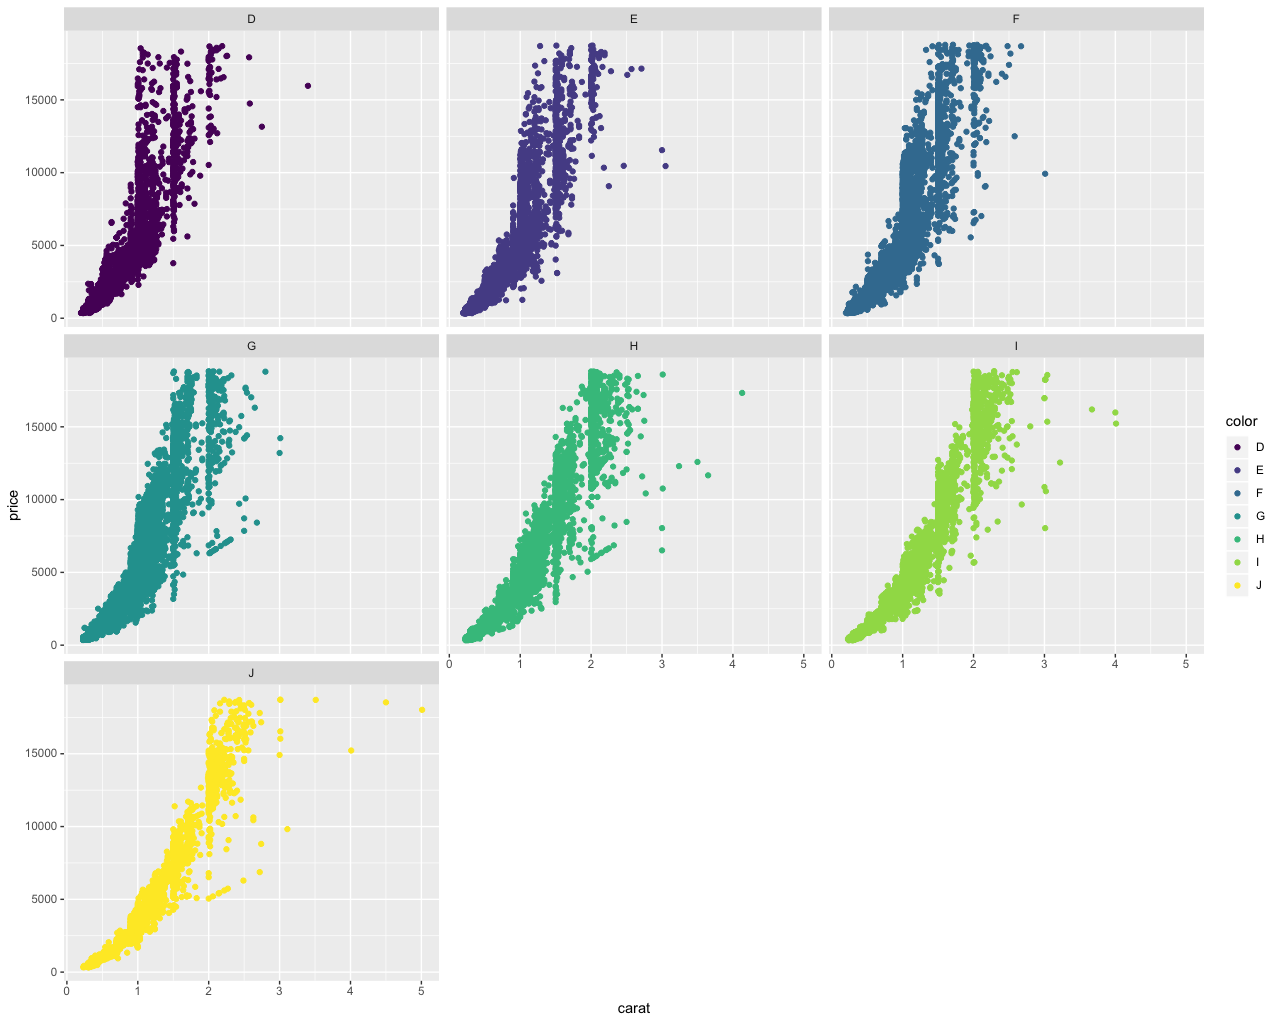
\includegraphics[width=1.0\linewidth]{pic0034}
  \caption{Диаграма на разпръскване по групи за цвят на диамантите}
\label{figure0034}
\end{figure}
\FloatBarrier

Функцията $facet\_grid$ действа по сходен начин, но всички стойности на признака за групиране се отразяват на осите за всяка от графиките (Фиг. \ref{figure0035}). Важно е да се забележи начина по който са ориентирани осите на всяка от подграфиките. Ориентацията пряко зависи дали признакът за чистота е от ляво, а признакът за качество на среда от дясно или обратното. 

\begin{figure}[h!]
  \centering
  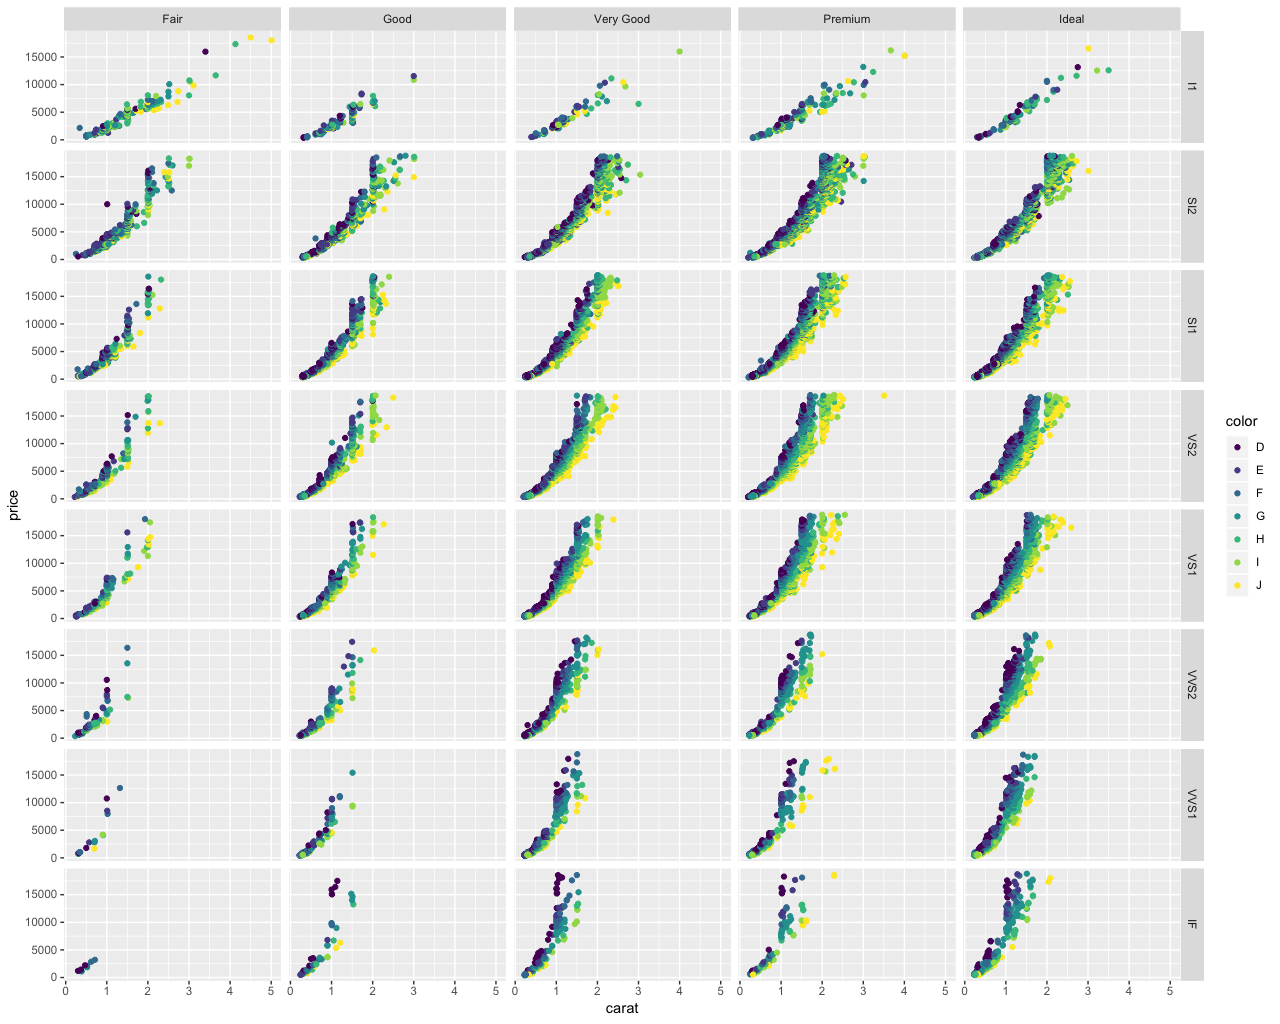
\includegraphics[width=1.0\linewidth]{pic0035}
  \caption{Визуализация с групиране по два признака}
\label{figure0035}
\end{figure}
\FloatBarrier

Организацията на графики по групи е възможна с различни графични представяния, като пример е представянето на хистограма\index{хистограма} в групи по качество на сряза (Фиг. \ref{figure0036}).

\begin{figure}[h!]
  \centering
  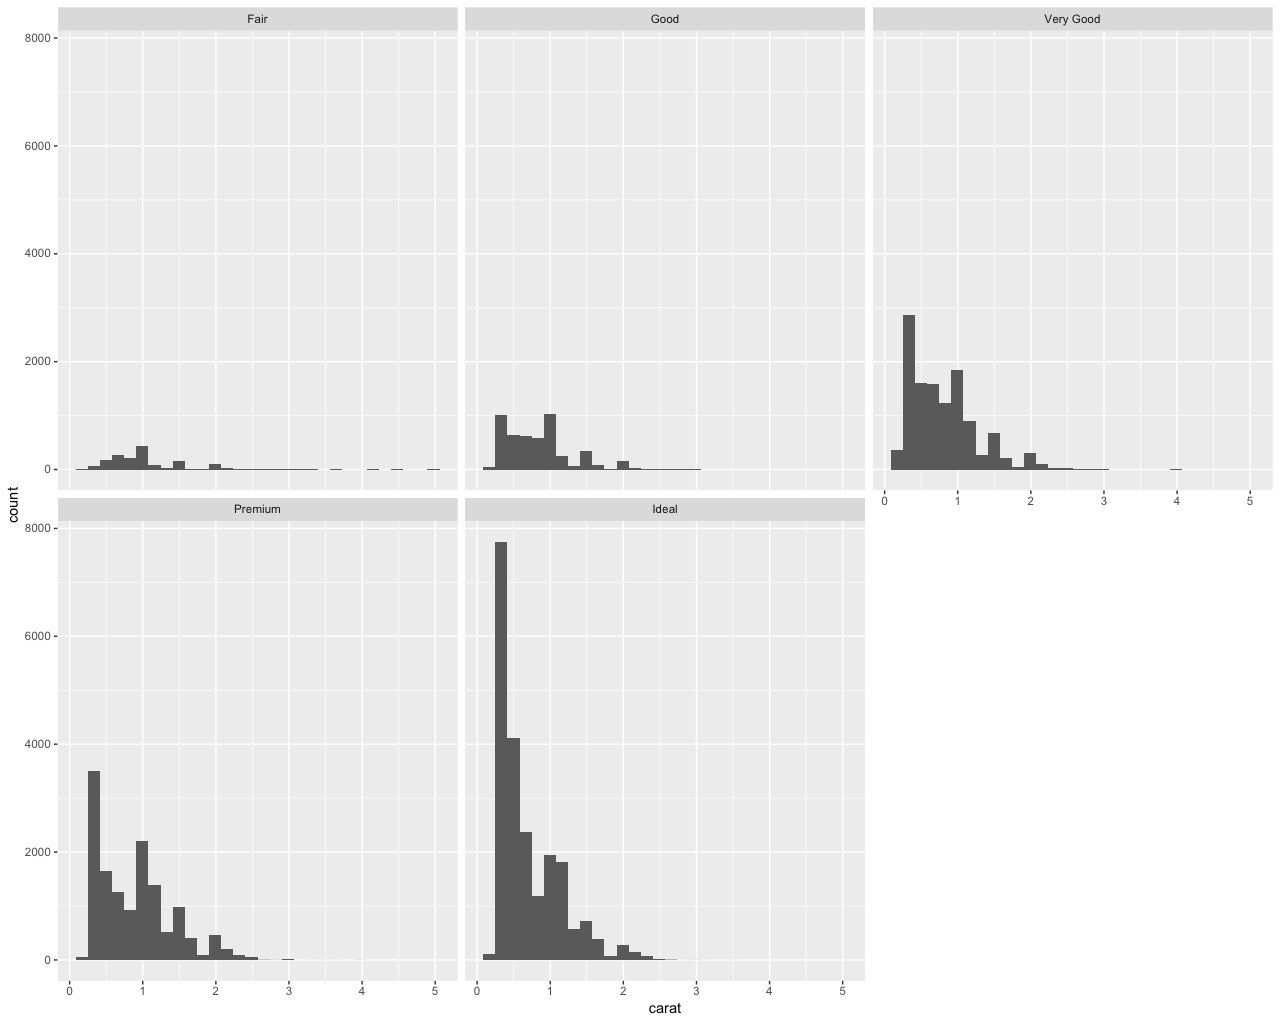
\includegraphics[width=1.0\linewidth]{pic0036}
  \caption{Визуализация на хистограми с групиране}
\label{figure0036}
\end{figure}
\FloatBarrier

\subsection{Графики тип кутия и цигулка}

Пакетът $ggplot2$ дава възможност за визуализация на графики тип кутия\index{графика тик кутия} (Листинг \ref{listing0153}).

\begin{lstlisting}[caption=Визуализация тип кутия, label=listing0153]
ggplot(diamonds, aes(y=depth)) + geom_boxplot()

ggplot(diamonds, aes(y=depth, x=cut)) + geom_boxplot()

ggplot(diamonds, aes(y=depth, x=cut)) + geom_boxplot() + geom_violin()

ggplot(diamonds, aes(y=depth, x=cut))+ geom_point() + geom_violin()
\end{lstlisting}

При обща визуализация на данните, без да се търси групиране по признан за абсцисната ос може да не се подава стойност (Фиг. \ref{figure0037}). 

\begin{figure}[h!]
  \centering
  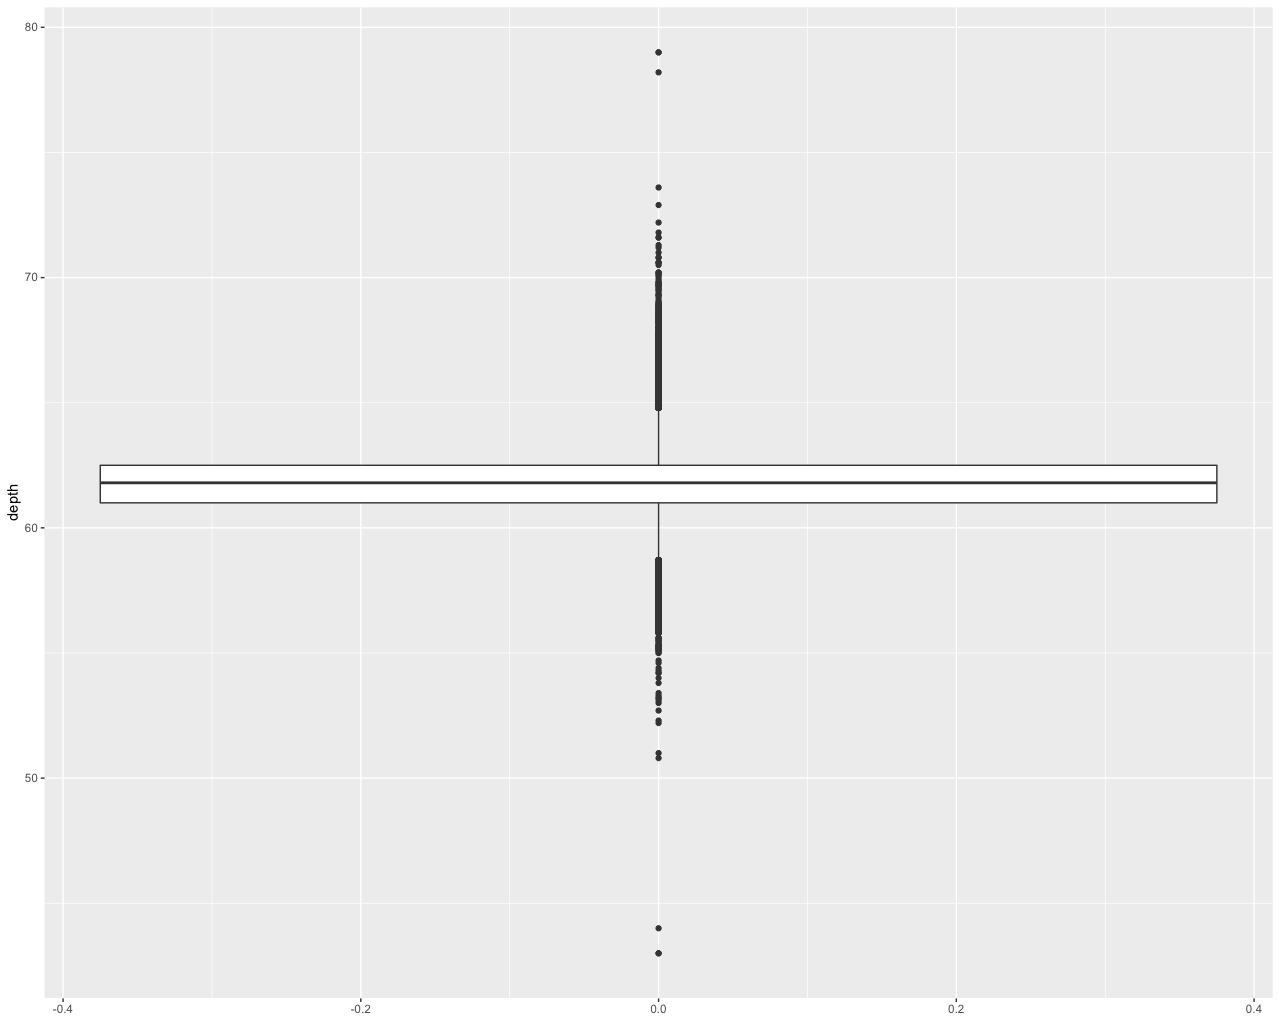
\includegraphics[width=1.0\linewidth]{pic0037}
  \caption{Визуализация на характеристиката за дълбочина на диамантите}
\label{figure0037}
\end{figure}
\FloatBarrier

Визуализацията на графики от тип кутия, с групиране по признак се реализира чрез подаване на колоната, по която да се групира, като параметър за абцисна ос, на функцията aes (Фиг. \ref{figure0038}).

\begin{figure}[h!]
  \centering
  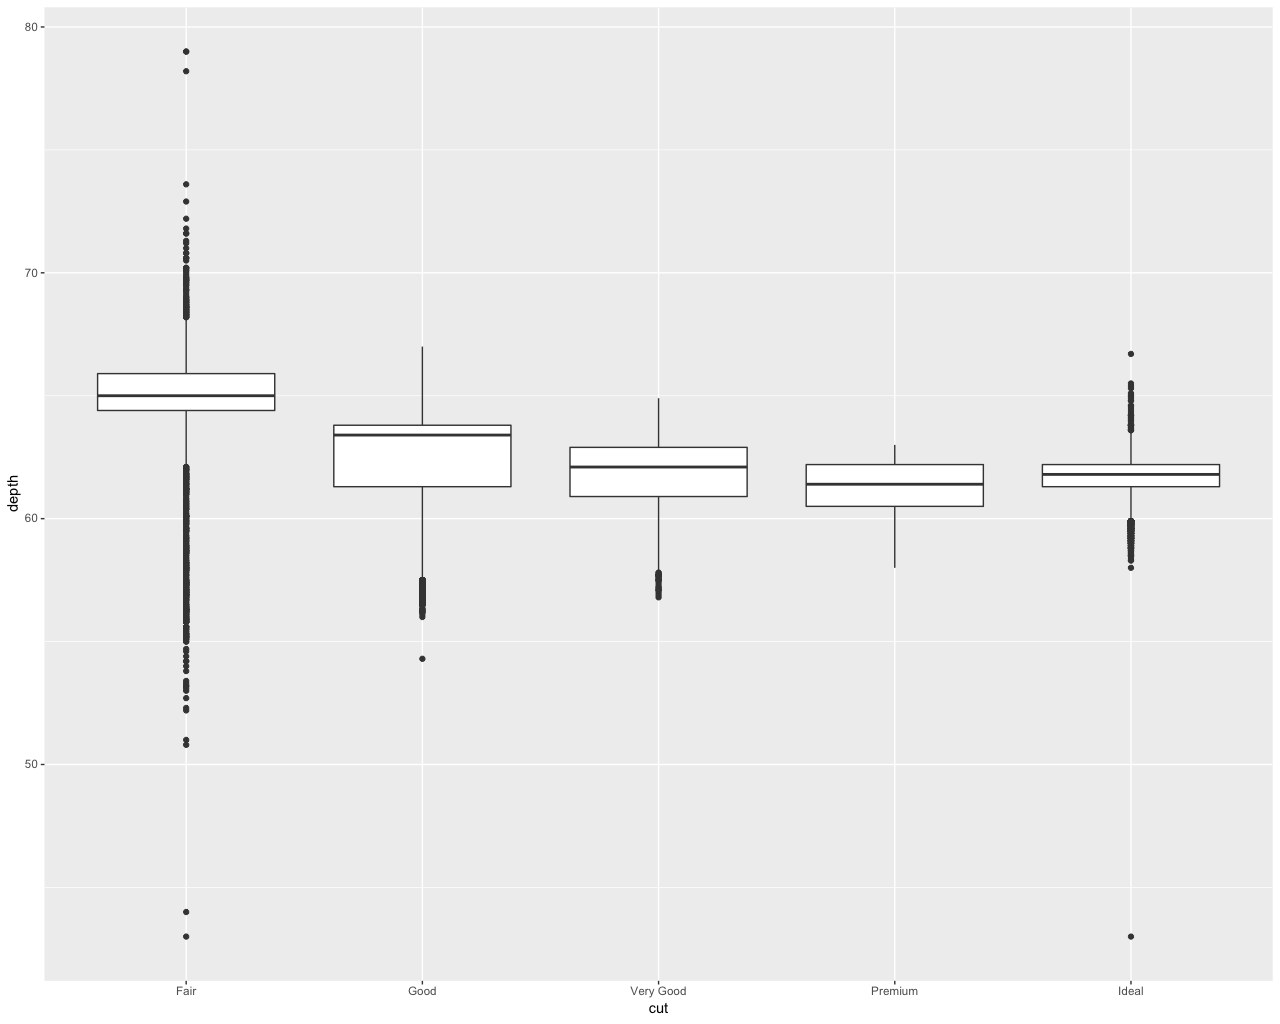
\includegraphics[width=1.0\linewidth]{pic0038}
  \caption{Dълбочина на диамантите в групи според сряза}
\label{figure0038}
\end{figure}
\FloatBarrier

От графика тип кутии много лесно се преминава към графика от тип цигулки\index{графика тип цигулка}, чрез подмяна на декориращата функция (Фиг. \ref{figure0039}).

\begin{figure}[h!]
  \centering
  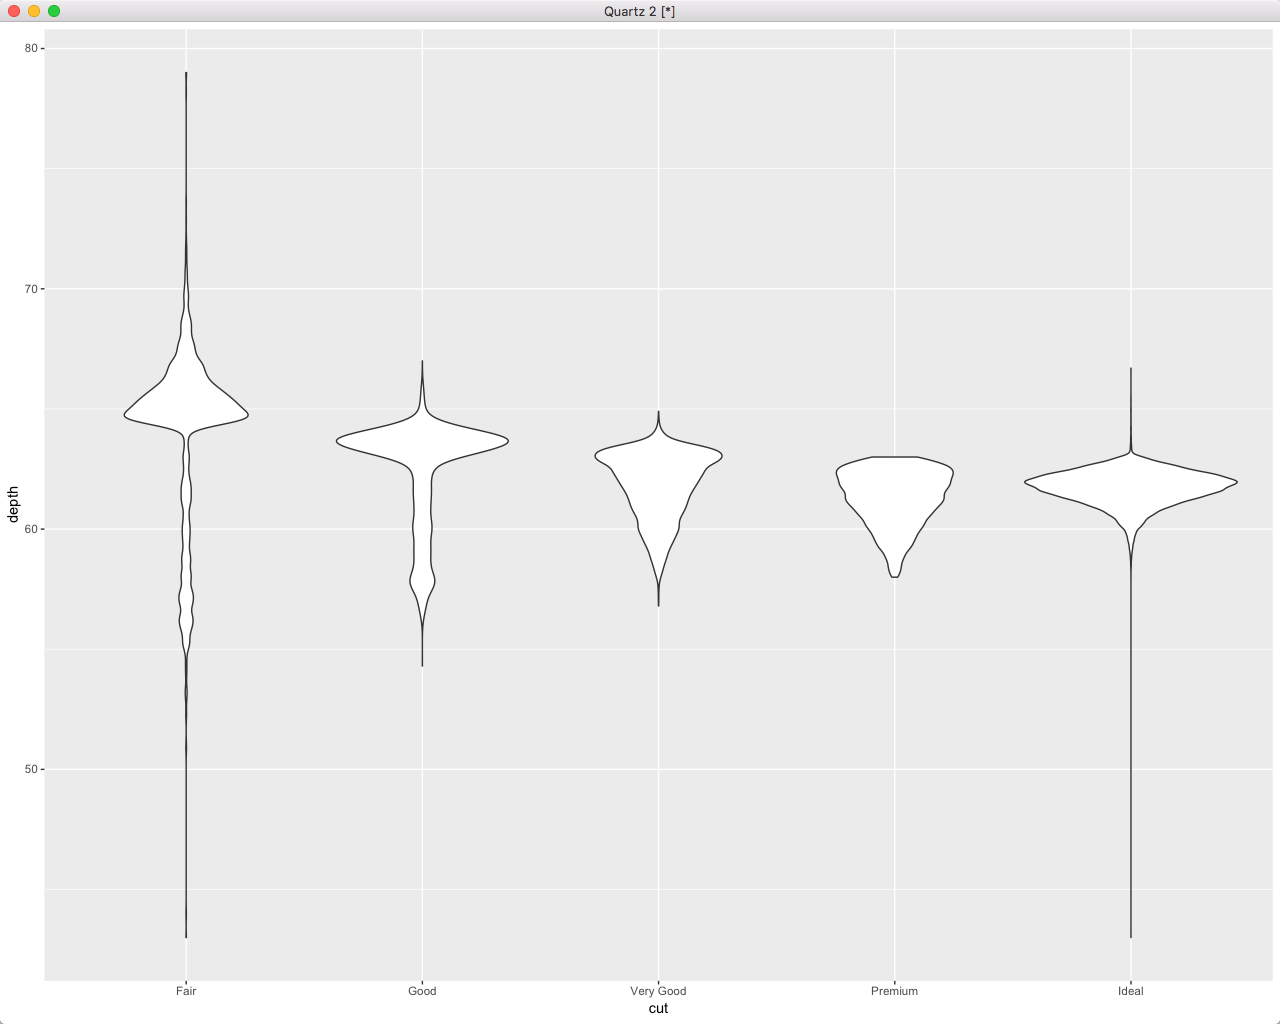
\includegraphics[width=1.0\linewidth]{pic0039}
  \caption{Графика тип цигулки}
\label{figure0039}
\end{figure}
\FloatBarrier

Графиките тип кутия и тип цигулка си приличат, като основната разлика е, че цигулките имат повече смисъла на плътностна функция и носят повече информация, отколкото правите ръбове на кутиите. 

\begin{figure}[h!]
  \centering
  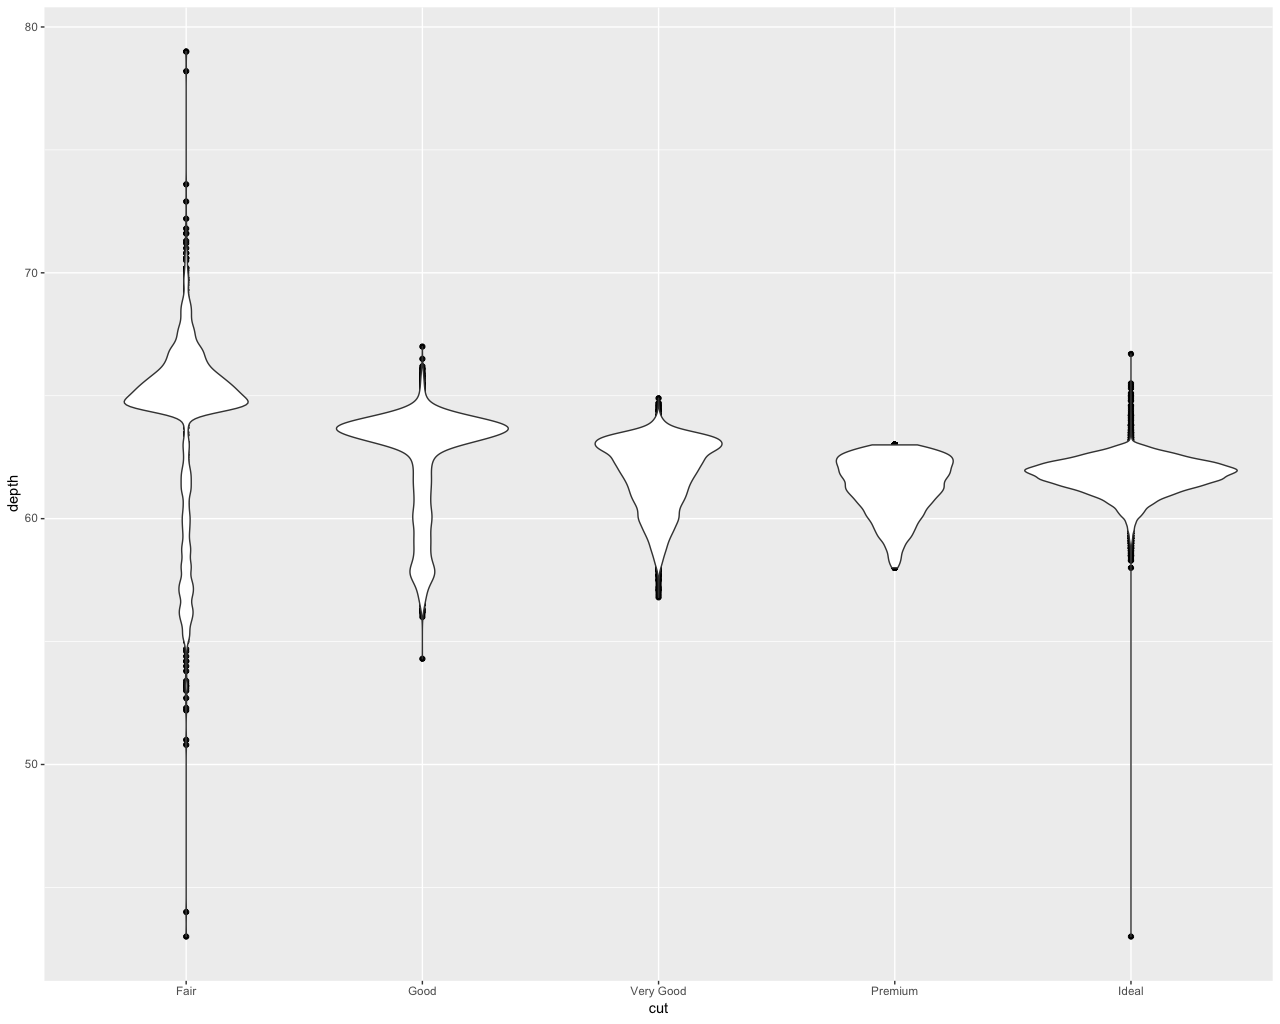
\includegraphics[width=1.0\linewidth]{pic0040}
  \caption{Добавяне на декорация с точки}
\label{figure0040}
\end{figure}
\FloatBarrier

Декорациите за визуализация на данните може да се наслагват една върху друга, като от съществено значение е редът на изчертаването им (Фиг. \ref{figure0040}). Ако декорацията с точките бъде добавена след декорацията с цигулките, точки ще се появят и върху самите цигулки. 

\subsection{Линейни графики}

В определени случаи най-удачно е визуалното представяне на информацията да бъде извършено с линейни графики\index{линейна графика}. Линейната графика е удачна примерно при представянето на тренд (Листинг \ref{listing0154}).

\begin{lstlisting}[caption=Линейни графики, label=listing0154]
library(lubridate)

ggplot(economics, aes(x=date, y=pop)) + geom_line()

economics$year <- year(economics$date)
economics$month <- month(economics$date, label=TRUE)

library(scales)

ggplot(economics, aes(x=month, y=pop)) + geom_line(aes(color=factor(year), group=year)) + scale_color_discrete(name="Year") + scale_y_continuous(labels=comma)+ labs(title="Population Growth", x="Month", y="Population")
\end{lstlisting}

В примерните данни за икономическо развитие, нарастването на популацията във времето е представена под формата на линейна графика (Фиг. \ref{figure0041}).

\begin{figure}[h!]
  \centering
  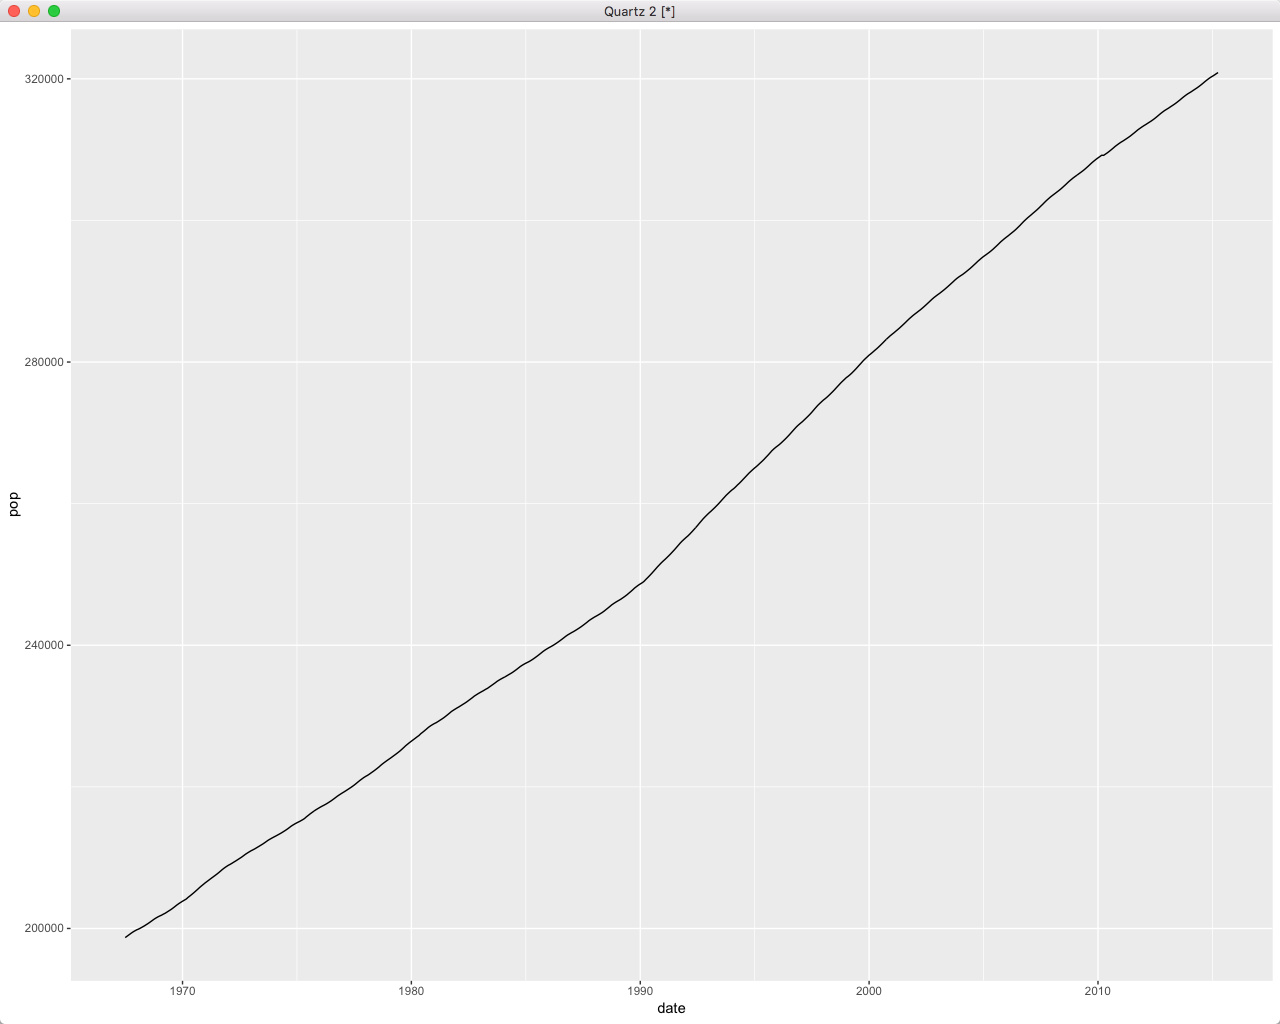
\includegraphics[width=1.0\linewidth]{pic0041}
  \caption{Нарастване на популацията във времето}
\label{figure0041}
\end{figure}
\FloatBarrier

При анализирането на ръст в популацията понякога е интересно тази информация да се организира по години и да се представи в обща графика. Данните за всяка година могат да се представят с различен цвят, така че да бъде ясно кои линии за кои периоди от време се отнасят. С помощта на библиотеката $lubridate$ в $economics$ данните се добавят две допълнителни колони за година и за месец. С помощта на библиотеката $scales$ се постига по-добро оформление на информацията по осите. 

\begin{figure}[h!]
  \centering
  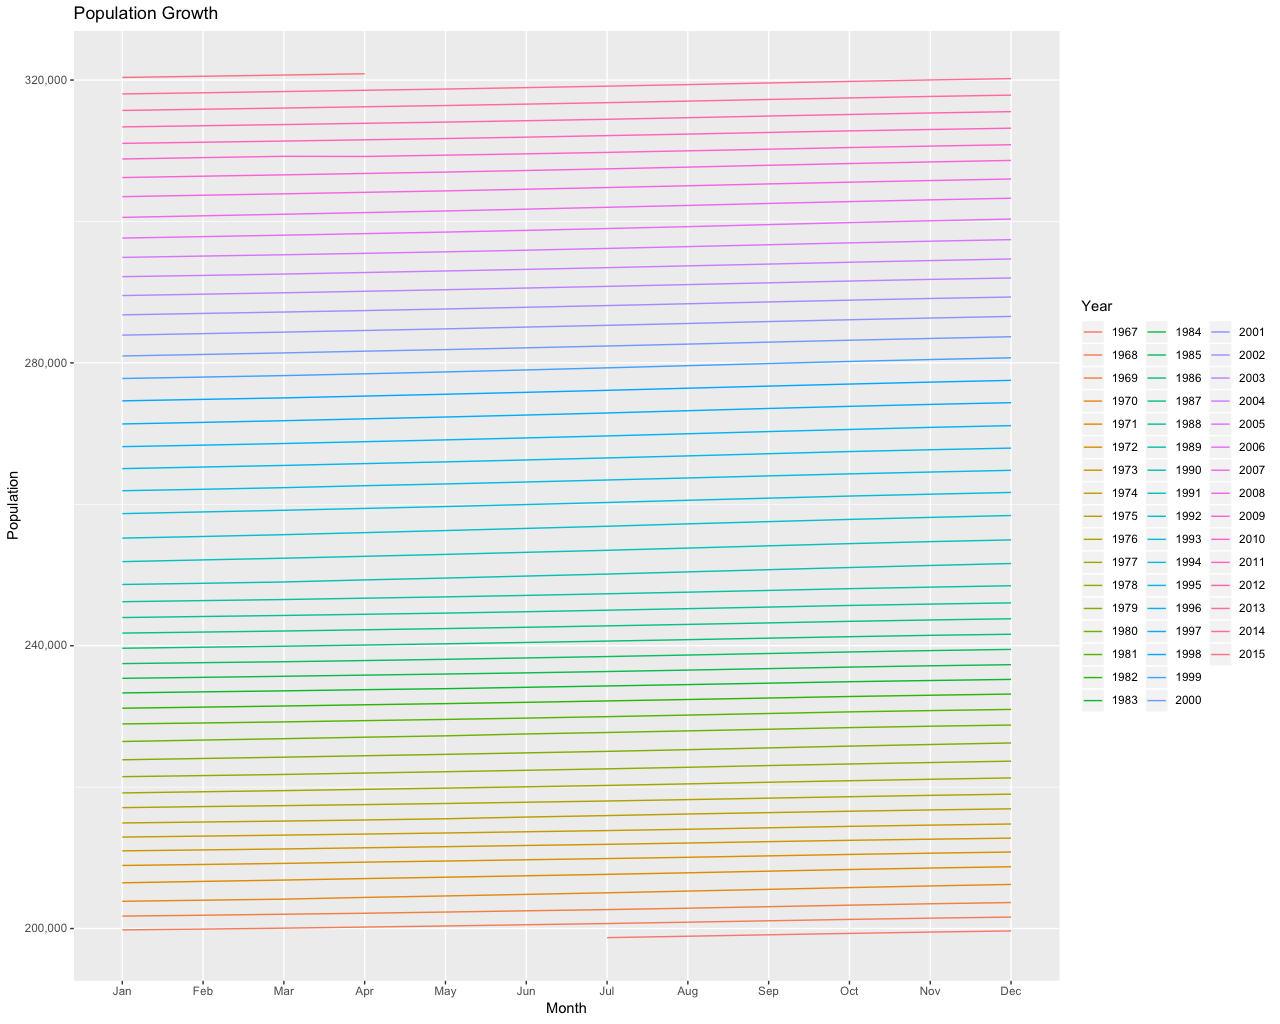
\includegraphics[width=1.0\linewidth]{pic0042}
  \caption{Визуализиране на приръста по години}
\label{figure0042}
\end{figure}
\FloatBarrier

Важно е да се отбележи, че информацията за годината е от тип $factor$, така че да се използва за определяне на цветовете. Също така на ординатната ос се добавя и запетая, като разделител за хилядите. Като последна декорация е подмяната на текстовете за двете оси. 

\subsection{Тематично оформление}

При генерирането на графики е от съществено значение медията на която тези графики ще бъдат представяни. При визуализация на проектор или монитор може да се използват тематично тъмни\index{графични теми} цветове, а при разпечатване на хартия е по-разумно да се използват светли цветове, така че да се намалява разхода на мастило (Листинг \ref{listing0155}). Каквито и да са нуждите за представяне, в пакетът $ggthemes$ са добавени възможности за цялостно преобразяване на получените графики, чрез избор на теми (Фиг. \ref{figure0043}-\ref{figure0046}).

\begin{lstlisting}[caption=Избор на теми за визуално представяне, label=listing0155]
library(ggthemes)

ggplot(diamonds, aes(x=carat, y=price)) + geom_point(aes(color=color)) + theme_wsj()

ggplot(diamonds, aes(x=carat, y=price)) + geom_point(aes(color=color)) + theme_tufte()

ggplot(diamonds, aes(x=carat, y=price)) + geom_point(aes(color=color)) + theme_excel()

ggplot(diamonds, aes(x=carat, y=price)) + geom_point(aes(color=color)) +  theme_economist() + scale_colour_economist()
\end{lstlisting}

\begin{figure}[h!]
  \centering
  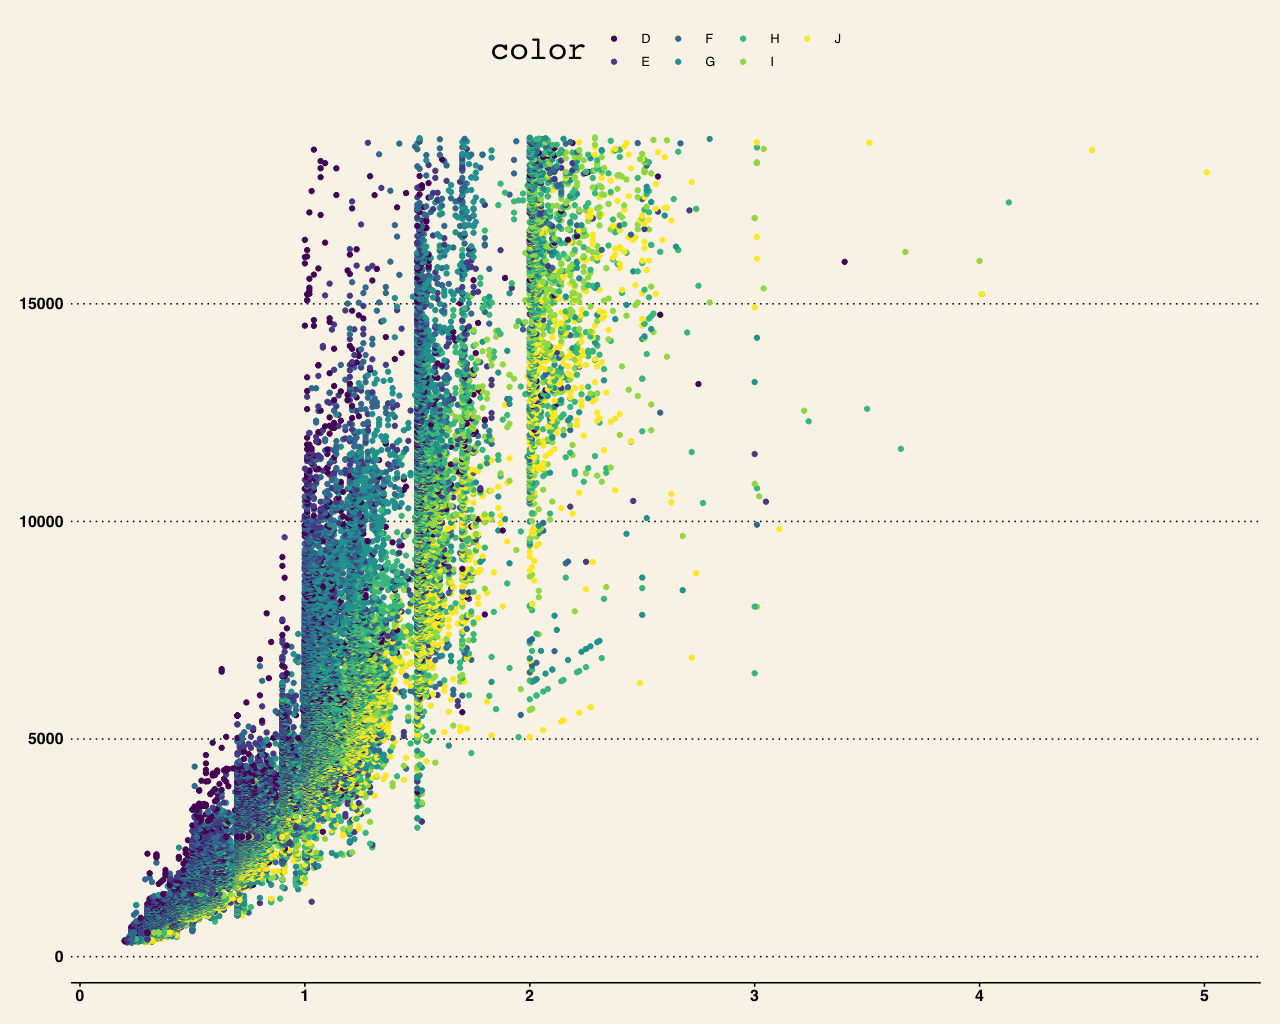
\includegraphics[width=1.0\linewidth]{pic0043}
  \caption{Тема Wall Street Journal}
\label{figure0043}
\end{figure}
\FloatBarrier

\begin{figure}[h!]
  \centering
  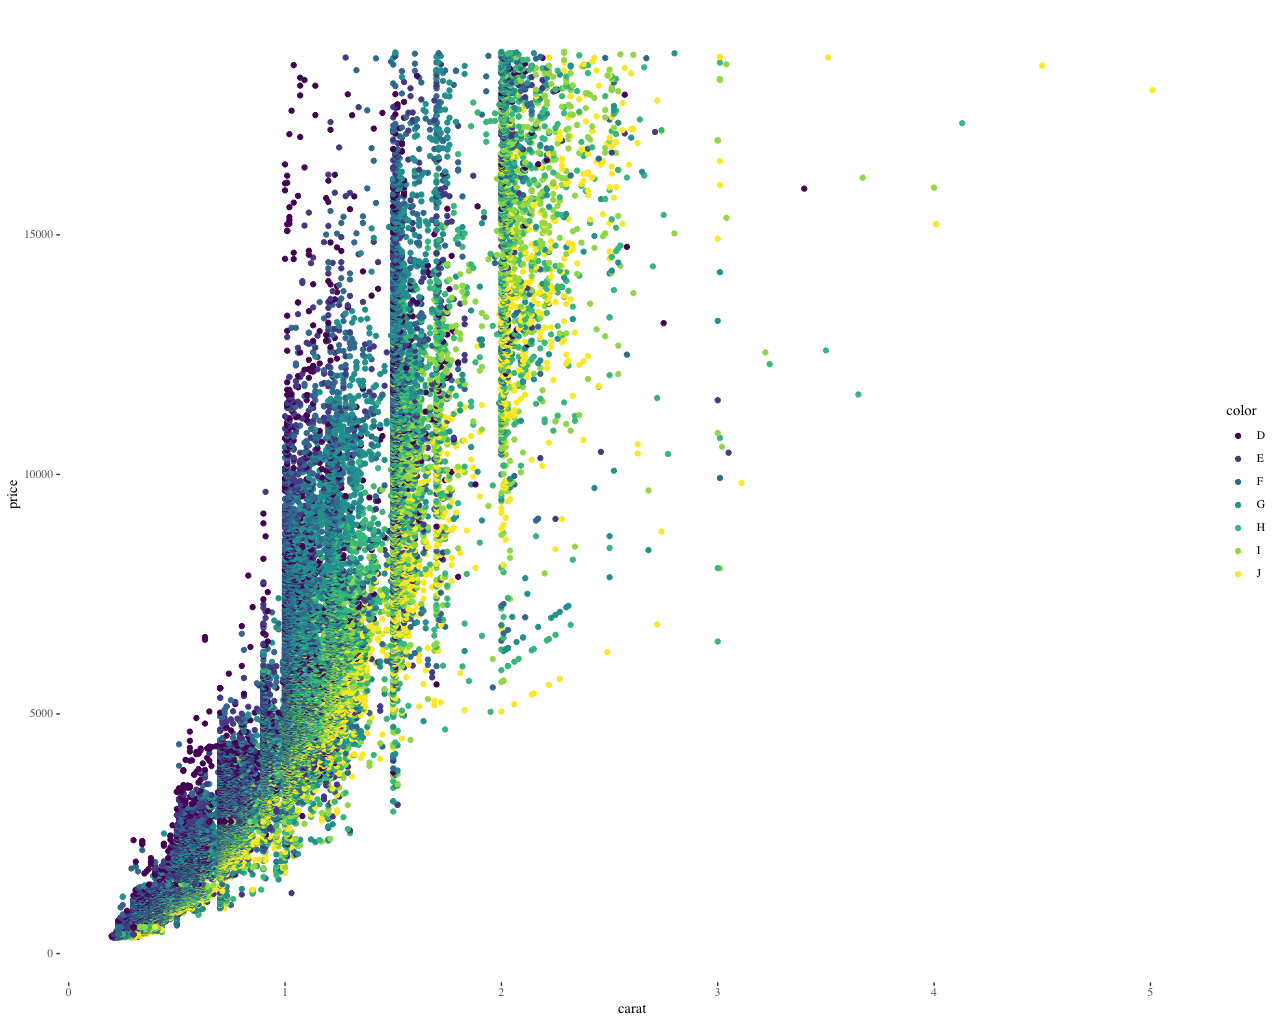
\includegraphics[width=1.0\linewidth]{pic0044}
  \caption{Тема Edward Tufte}
\label{figure0044}
\end{figure}
\FloatBarrier

\begin{figure}[h!]
  \centering
  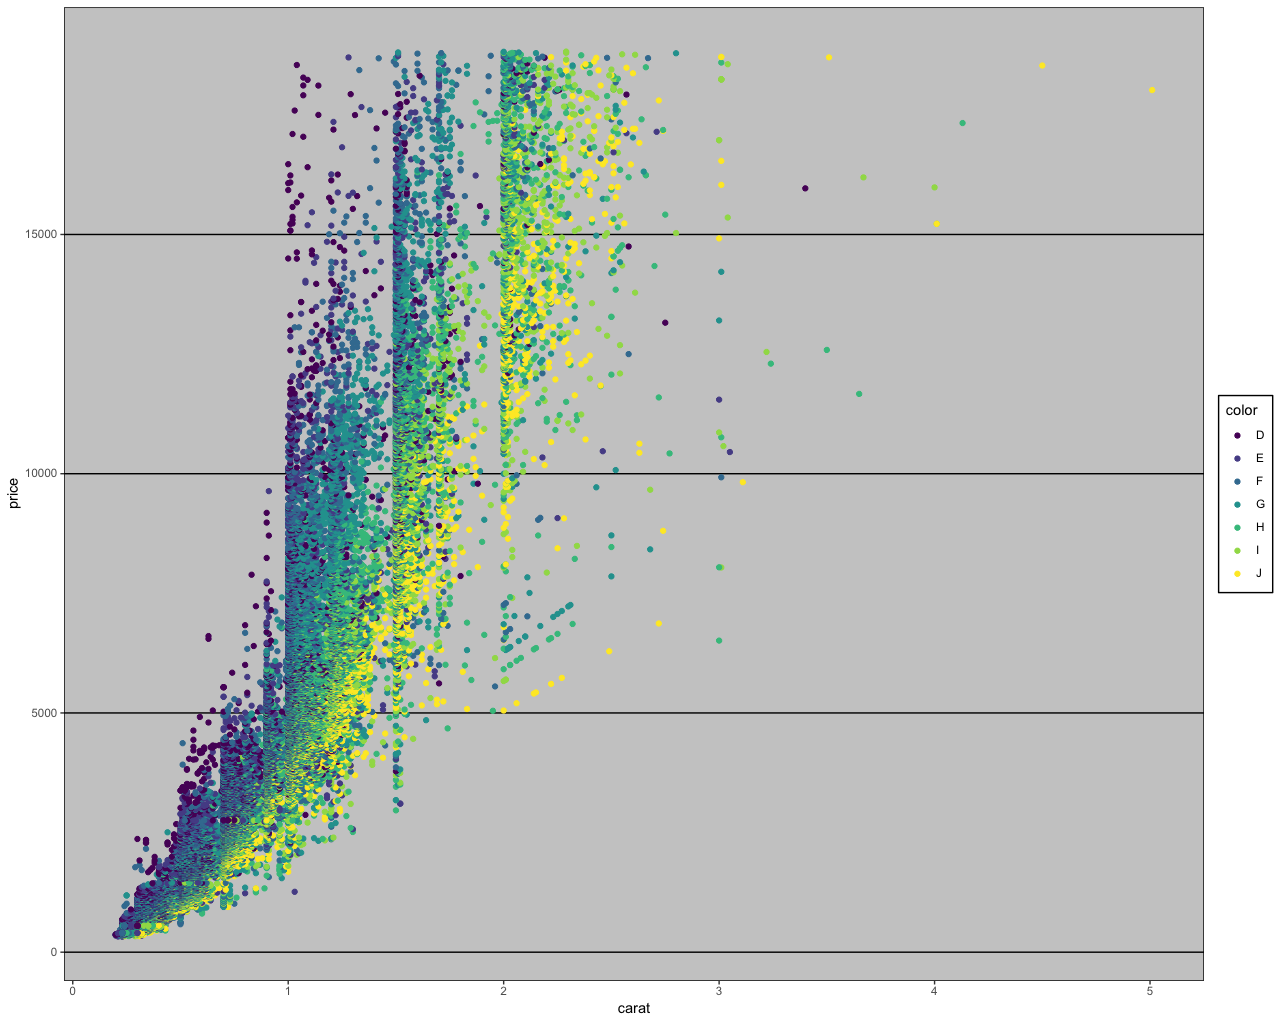
\includegraphics[width=1.0\linewidth]{pic0045}
  \caption{Тема в стил Microsoft Excel}
\label{figure0045}
\end{figure}
\FloatBarrier

\begin{figure}[h!]
  \centering
  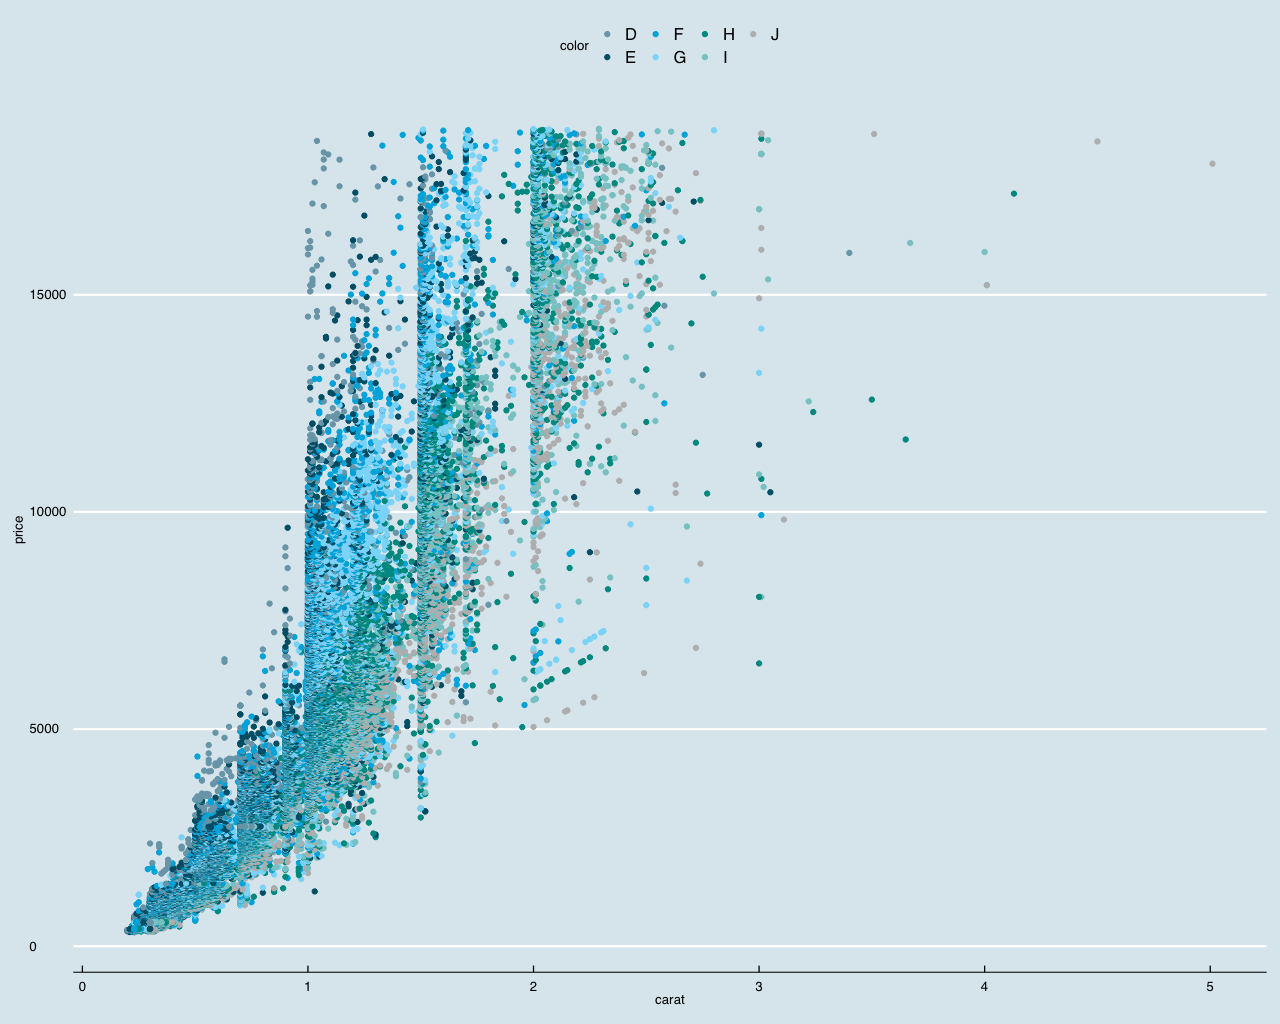
\includegraphics[width=1.0\linewidth]{pic0046}
  \caption{Тема Economist}
\label{figure0046}
\end{figure}
\FloatBarrier

\section{Изследване на случайни величини}

Когато се работи с данни за които няма предварителна информация е от съществено значение да се определи какви са параметрите на вероятностното разпределение. С помощта на пакета $Rdice$ е възможно да се генерират експерименти с различни зарове. Чрез генерирането и статистическото изследване на множество случайни събития се осъществява изследване наречено „Монте Карло метод“\index{метод Монте-Карло}.

\begin{lstlisting}[caption=Случайни величини със зарове, label=listing0156]
library(ggplot2)
library(Rdice)

x <- dice.roll(faces=6, dice=1, rolls=100000)

ggplot(data=x$results) + geom_histogram(aes(x=values)) + ggtitle("Single die rolled 100K times.") + xlab("Die Side") + ylab("Outcomes") + scale_x_continuous(breaks=round(seq(min(x$results$values),max(x$results$values),by=0.5)))

x <- dice.roll(faces=6, dice=2, rolls=100000)

ggplot(data=x$results) + geom_histogram(aes(x=(die_1+die_2))) + ggtitle("Two dice rolled 100K times.") + xlab("Dice Sides") + ylab("Outcomes") + scale_x_continuous(breaks=round(seq(min((x$results$die_1+x$results$die_2)),max((x$results$die_1+x$results$die_2)),by=0.5)))

x <- dice.roll(faces=6, dice=6, rolls=100000)
x$results$values = rowSums( x$results[,1:6] )

ggplot(data=x$results) + geom_histogram(aes(x=values)) + ggtitle("Six dice rolled 100K times.") + xlab("Dice Sides") + ylab("Outcomes") + scale_x_continuous(breaks=round(seq(min(x$results$values),max(x$results$values),by=0.5)))

x <- dice.roll(faces=6, dice=10, rolls=100000)
x$results$values = rowSums( x$results[,1:10] )

ggplot(data=x$results) + geom_density(aes(x=values)) + ggtitle("Ten dice rolled 100K times.") + xlab("Dice Sides") + ylab("Outcomes") + scale_x_continuous(breaks=round(seq(min(x$results$values),max(x$results$values),by=0.5)))
\end{lstlisting}

Ако се приеме, че променливата $x$ е резултатът от многократното хвърляне на един математически честен зар, със шест страни, то чрез изчертаване на хистограмата\index{хистограма} може да се добие представа за характера на случайната величина (Листинг \ref{listing0156}). От изчертаната хистограма ясно се вижда, че случайната величина е дискретна и равномерно разпределена (Фиг. \ref{figure0047}).

\begin{figure}[h!]
  \centering
  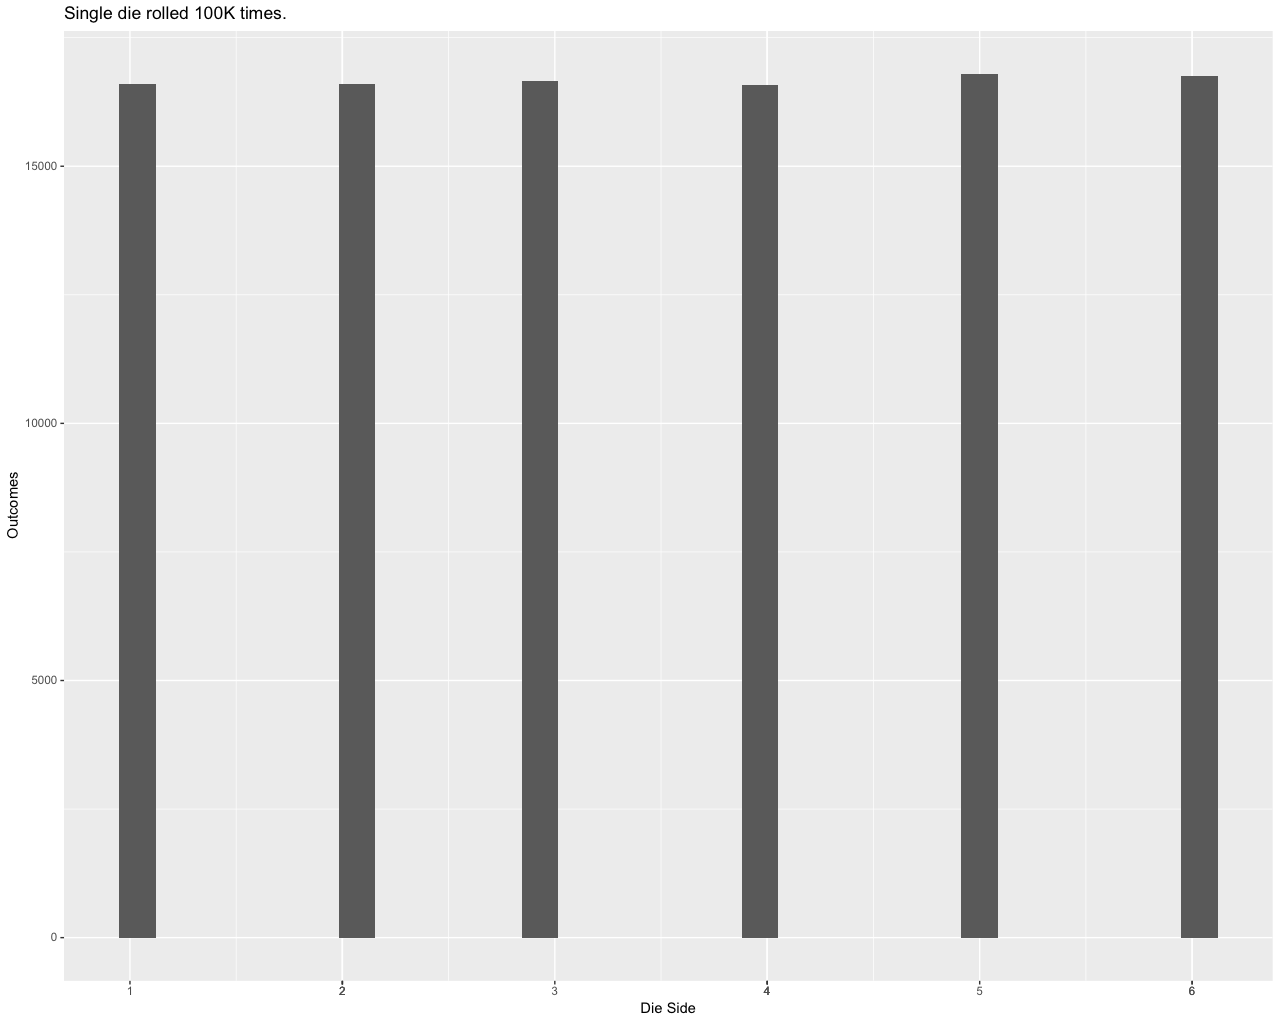
\includegraphics[width=1.0\linewidth]{pic0047}
  \caption{Хистограма на хвърлянията за един зар}
\label{figure0047}
\end{figure}
\FloatBarrier

Когато същият експеримент бъде повторен, но вместо един зар се използват два зара, ясно се различава, че някои събития стават по-малко вероятни от други и разпределението се превръща в триъгълно (Фиг. \ref{figure0048}).

\begin{figure}[h!]
  \centering
  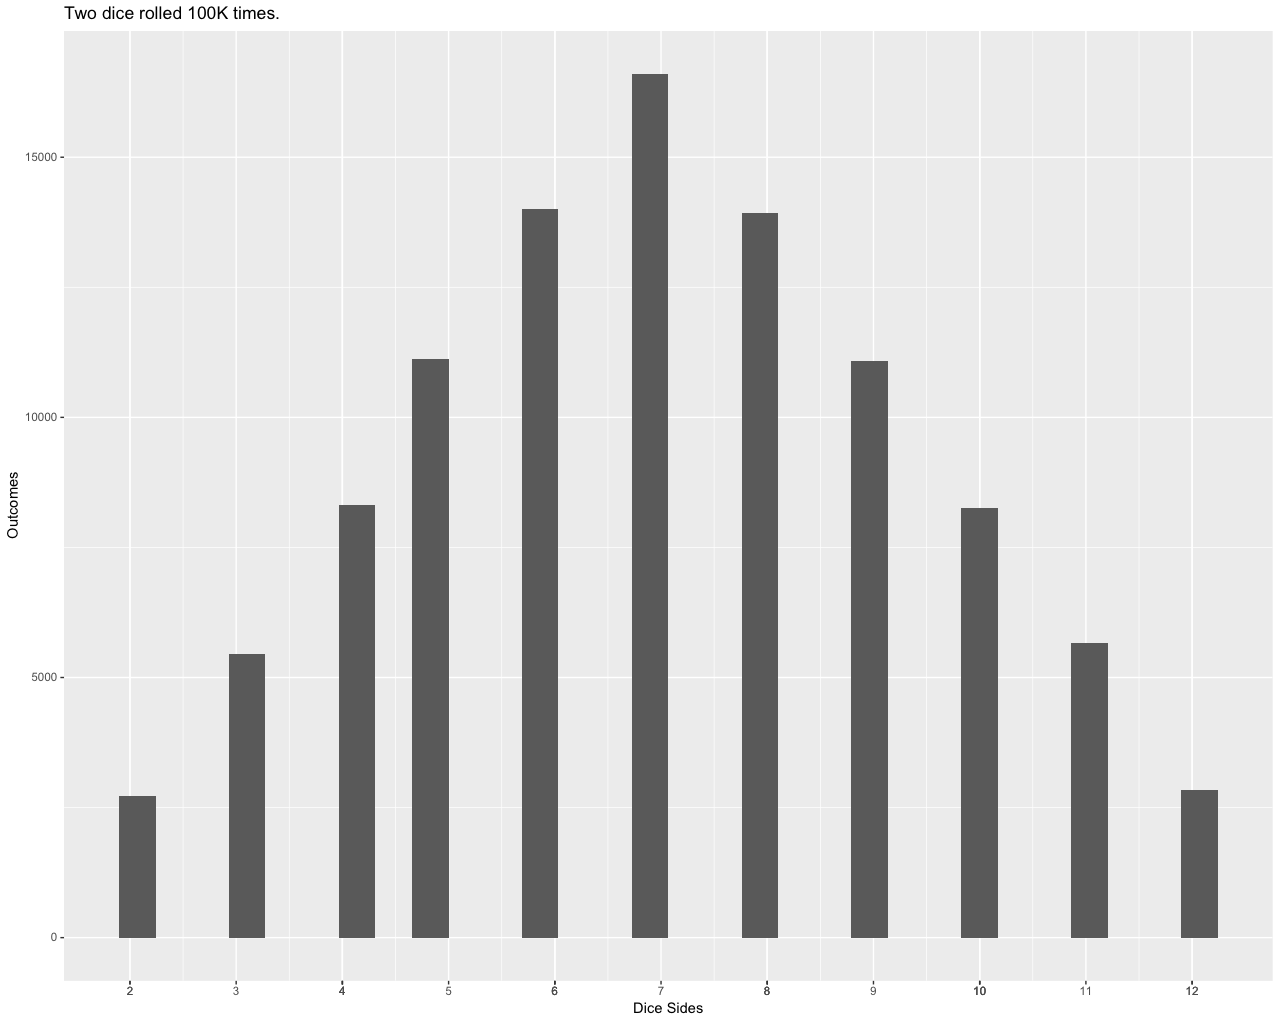
\includegraphics[width=1.0\linewidth]{pic0048}
  \caption{Хистограма на хвърлянията за два зара}
\label{figure0048}
\end{figure}
\FloatBarrier

При шест зара ясно започва да се различава формата на нормалното разпределение (Фиг. \ref{figure0049}).

\begin{figure}[h!]
  \centering
  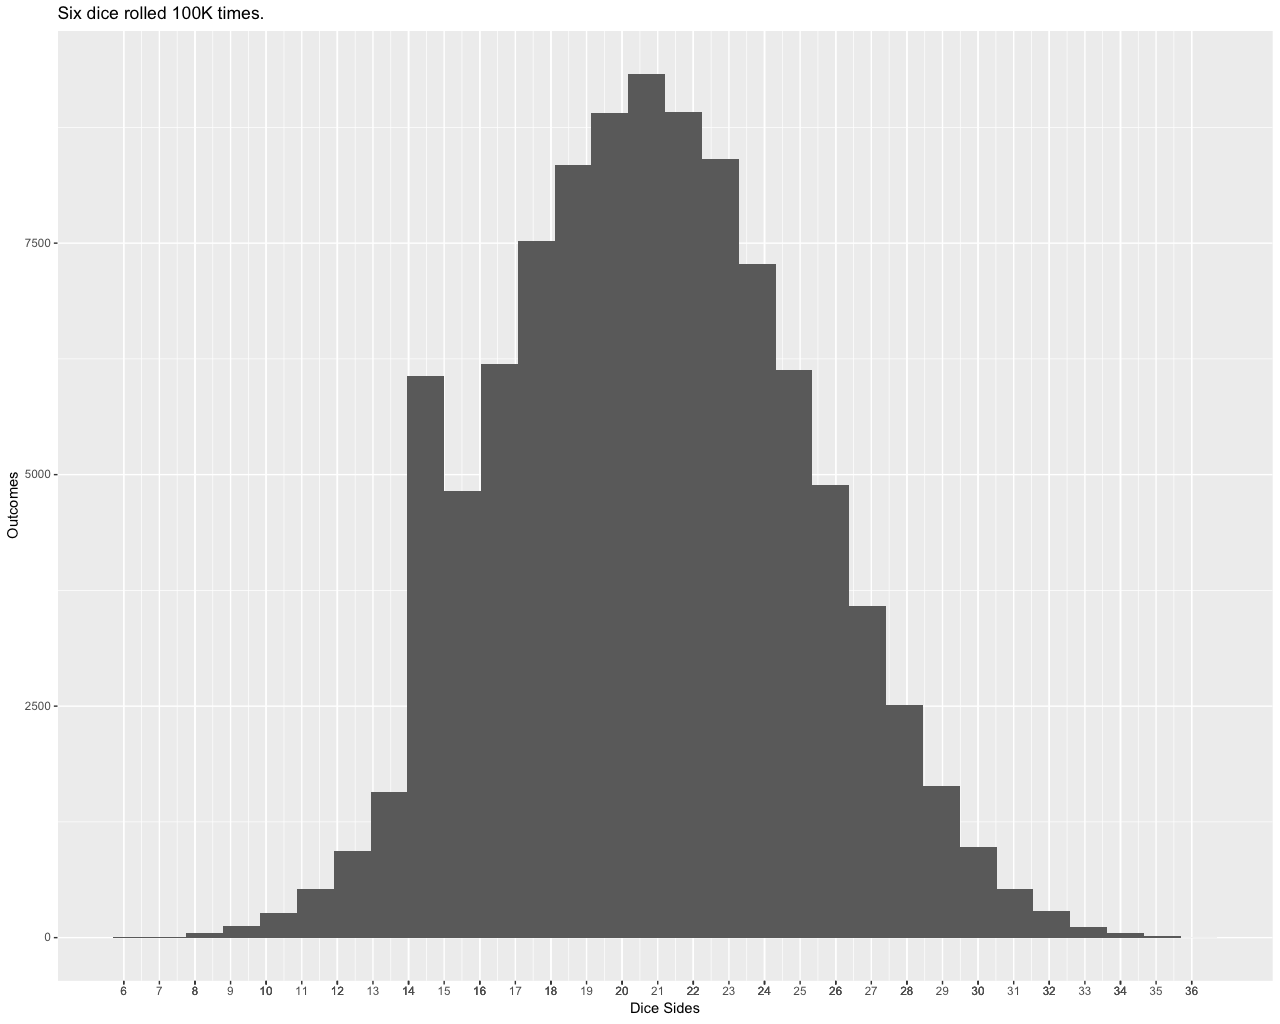
\includegraphics[width=1.0\linewidth]{pic0049}
  \caption{Хистограма на хвърлянията за шест зара}
\label{figure0049}
\end{figure}
\FloatBarrier

При десет зара и изчертаване на плътностна диаграма формата на нормалното вероятностно разпределение е ясно забележима (Фиг. \ref{figure0050}).

\begin{figure}[h!]
  \centering
  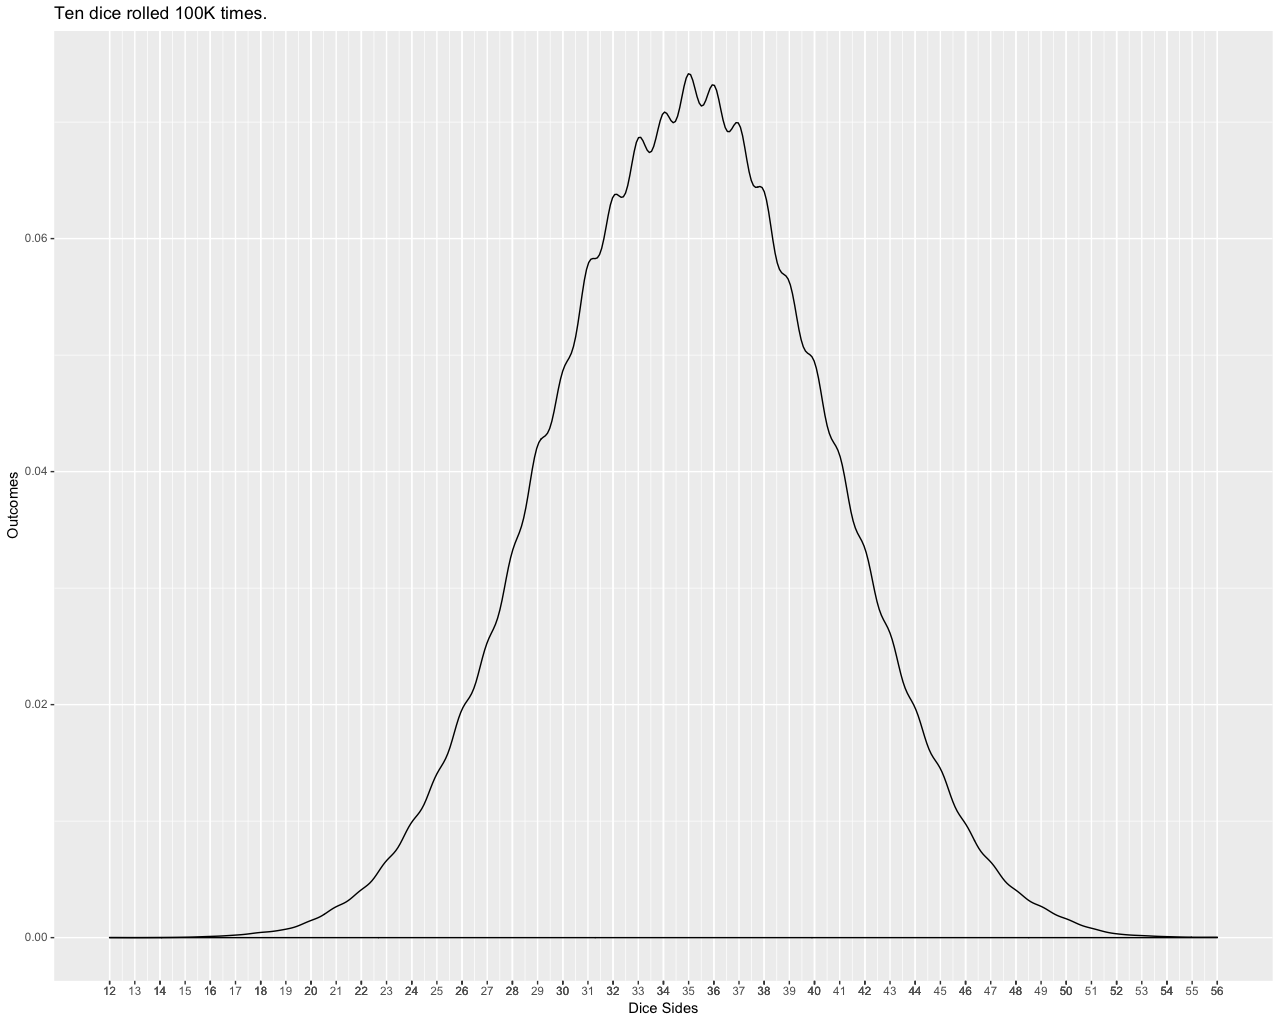
\includegraphics[width=1.0\linewidth]{pic0050}
  \caption{Плътностна диаграма на хвърлянията за десет зара}
\label{figure0050}
\end{figure}
\FloatBarrier

За изследването на една случайна величина, хистограмата и плътностната диаграма носят първоначална ориентировъчна информация за характеристиките на величината.

\section{Вероятностни разпределения}

В реалната практика от статистическия анализ се наблюдават множество случайни величини, които винаги се подчиняват на някакво вероятностно разпределение\index{вероятностно разпределение}. Определянето на вероятностното разпределение, към което принадлежи случайната величина има изключително важна роля в адекватното и надеждно извършване на статистическия анализ. След определяне на вероятностното разпределение от съществена важност е и определянето на параметрите, които характеризират разпределението.  

\subsection{Нормално разпределение}

Най-често срещаното в природата и най-използваното в статистическия анализ е нормалното разпределение. Също така, познато е и под названието на Гаусово разпределение\index{нормално разпределение} (Формула \ref{equation0002}). 

\begin{equation}
pdf(x) = \frac{1}{{\sigma \sqrt {2\pi } }}e^{{{ - \left( {x - \mu } \right)^2 } \mathord{\left/ {\vphantom {{ - \left( {x - \mu } \right)^2 } {2\sigma ^2 }}} \right. \kern-\nulldelimiterspace} {2\sigma ^2 }}}
\label{equation0002}
\end{equation}
\listofequations{Вероятностна функция на нормално разпределение}

Нормалното разпределение се характеризира с два параметъра - средната стойност $\mu$ и стандартно отклонение $\sigma$. Формата на графиката с която се изобразява нормалното разпределение е като камбана. Средната стойност задава къде се намира върхът на камбаната, по оста $X$, а стандартното отклонение определя широчината на камбаната. 

\begin{lstlisting}[caption=Нормално разпределение, label=listing0157]
library(ggplot2)

values <- rnorm(n=30000, mean=0, sd=0.85)
density <- dnorm( values )
cumulative <- pnorm( values )
quantile <- qnorm( cumulative )

ggplot(data.frame(x=values, y=density)) + aes(x=x, y=y) + geom_line() + labs(x="Normally Distributed Random Values ", y="Density")

ggplot(data.frame(x=values, y=cumulative)) + aes(x=x, y=y) + geom_line() + labs(x="Normally Distributed Random Values ", y="Cumulative Probability")

ggplot(data.frame(x=values, y=quantile)) + aes(x=x, y=y) + geom_line() + labs(x="Normally Distributed Random Values ", y="Quantile")
\end{lstlisting}

В езика R генерирането на нормално разпределени случайни числа става чрез функцията $rnorm$, която получава параметър за брой числа, средна стойност и стандартно отклонение. Подразбиращата се средна стойност е нула, а подразбиращото се стандартно отклонение е единица. Вероятността дадена стойност да бъде генериране се изчислява с функцията $dnorm$, която е полезна при изчертаването на плътностната функция (Фиг. \ref{figure0051}).

\begin{figure}[h!]
  \centering
  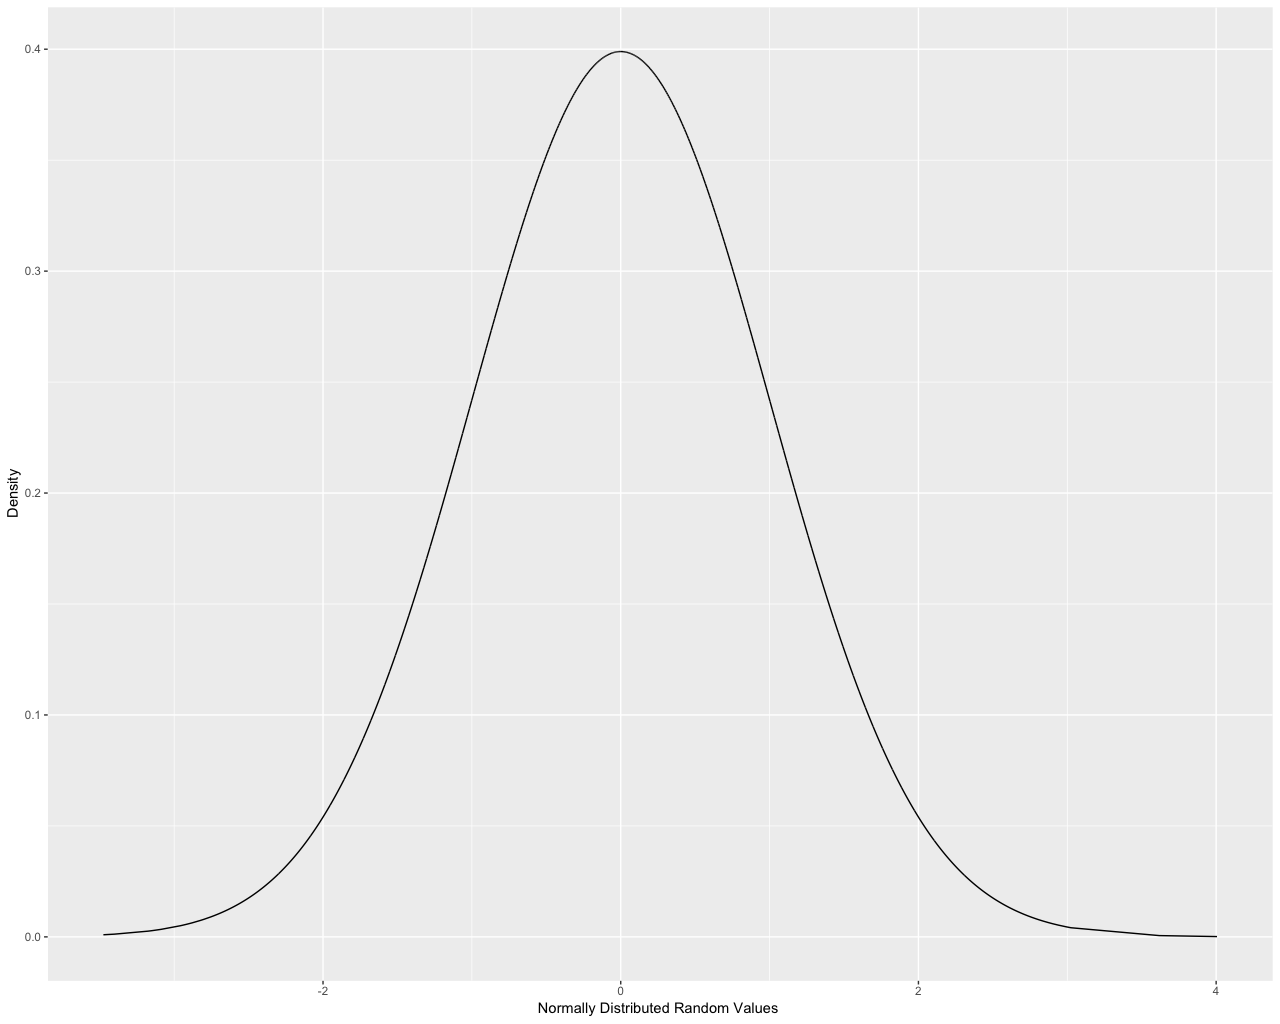
\includegraphics[width=1.0\linewidth]{pic0051}
  \caption{Плътностна функция на нормално разпределение}
\label{figure0051}
\end{figure}
\FloatBarrier

От плътностната функция\index{плътностна функция}, чрез интегриране, се получава кумулативната функция\index{кумулативна функция} на разпределението (Формула \ref{equation0003}).

\begin{equation}
cdf(x) = \int_{-\infty}^{a} \frac{1}{{\sigma \sqrt {2\pi } }}e^{{{ - \left( {x - \mu } \right)^2 } \mathord{\left/ {\vphantom {{ - \left( {x - \mu } \right)^2 } {2\sigma ^2 }}} \right. \kern-\nulldelimiterspace} {2\sigma ^2 }}} dx
\label{equation0003}
\end{equation}
\listofequations{Кумулативна функция на нормално разпределение}

Смисълът на кумулативната функция е, че определя вероятността да се падне число по-малко от зададеното в интервала (Фиг. \ref{figure0052}).

\begin{figure}[h!]
  \centering
  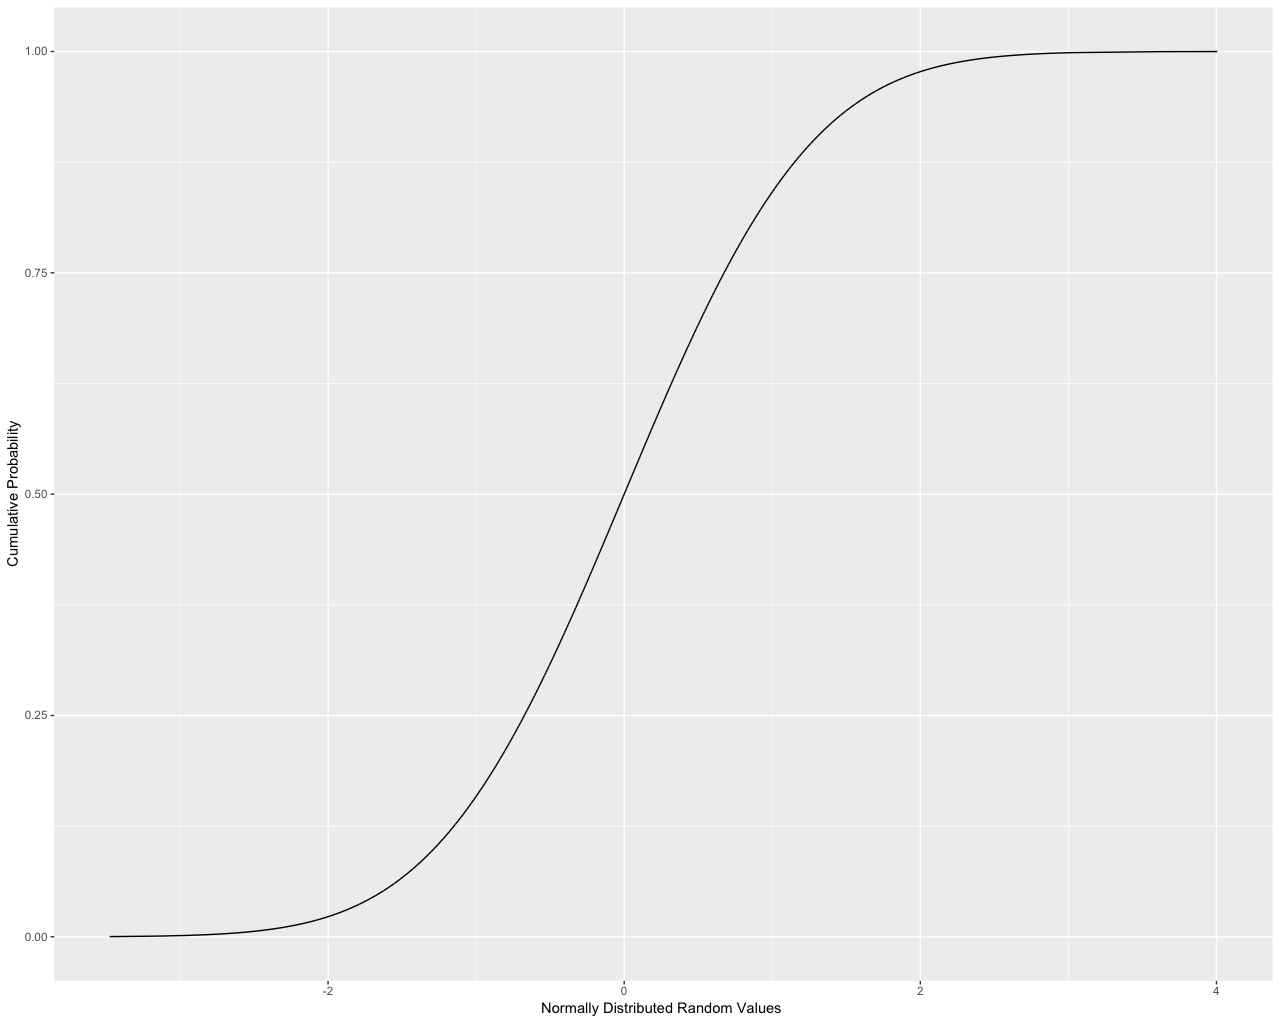
\includegraphics[width=1.0\linewidth]{pic0052}
  \caption{Комулативна функция на нормално разпределение}
\label{figure0052}
\end{figure}
\FloatBarrier

Обратната функция на $pnorm$ е $qnorm$ и тя изчислява квантила, ако е известна кумулативната вероятност.

\subsection{Биномно разпределение}

Биномното разпределение\index{биномно разпределение} (Формула \ref{equation0004}) е добре представено в R с помощта на серия функции по аналогия с функциите за нормално разпределение. 

\begin{equation}
pdf(x) = \binom{n}{x}p^{x}(1-p)^{n-x}
\label{equation0004}
\end{equation}
\listofequations{Вероятностна функция на биномно разпределение}

Където първият множител е биномен коефициент\index{биномни коефициенти} изчисляван по Формула \ref{equation0005}.

\begin{equation}
\binom{n}{x} = \frac{n!}{x!(n-x)!}
\label{equation0005}
\end{equation}
\listofequations{Биномен коефициент}

Параметърът $n$ определя броя опити, а параметърът $p$ задава вероятността за успех при единичен опит. Средната на биномното разпределение е $np$, а вариацията $np(1-p)$. Когато параметърът $n$ има стойност единица биномното разпределение се трансформира в бернулиево разпределение\index{бернулиево разпределение}. 

\begin{lstlisting}[caption=Биномно разпределение, label=listing0158]
library(ggplot2)

values <- rbinom(n=10000, size=7, prob=0.35)
density <- dbinom(x=2, size=7, prob=0.35)
cumulative <- pbinom(q=2, size=7, prob=0.35)
quantile <- qbinom(p=0.15, size=7, prob=0.35)

ggplot(data.frame(x=values)) + aes(x=x) + geom_histogram() + labs(x="Binomial Distributed Random Values ", y="Count")

density
cumulative
quantile
\end{lstlisting}

При биномното разпределение не просто се генерират случайни числа, а се генерират броя на успешните независими бернулиеви експеримента. В езика R за да се генерират биномно разпределени нормални числа се използва функцията $rbinom$ (Листинг \ref{listing0158}). Биномното разпределение е дискретно вероятностно разпределени, тъй като отразява определен брой успешни изходи от експеримент с предварително зададена вероятност за успех. Поради тази причина визуализацията става с помощта на хистограма (Фиг. \ref{figure0053}).

\begin{figure}[h!]
  \centering
  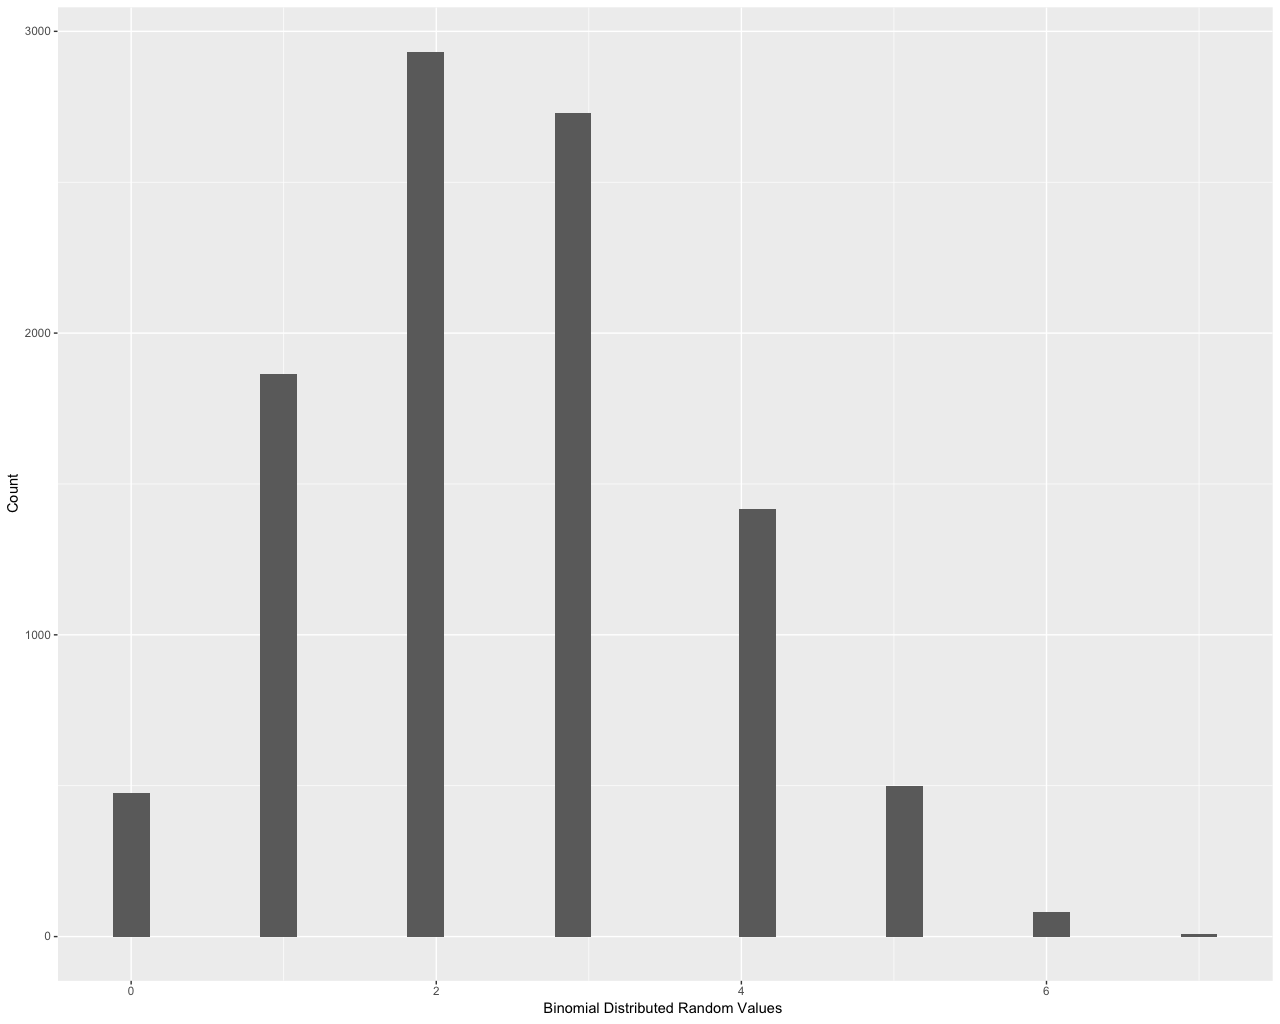
\includegraphics[width=1.0\linewidth]{pic0053}
  \caption{Хистограма на биномно разпределение}
\label{figure0053}
\end{figure}
\FloatBarrier

Освен броя случайни числа които трябва да се генерират към функцията $rbinom$ се подава параметър за броя експерименти и параметър за вероятността на успех при единичен експеримент. При значително увеличаване на броя експерименти биномното разпределение започва да клони към нормално разпределение. 

\begin{equation}
cdf(x) = \sum_{i=0}^{a}\binom{n}{i}p^{i}(1-p)^{n-i}
\label{equation0006}
\end{equation}
\listofequations{Кумулативна функция на биномно разпределение}

С функцията dbinom може да се провери плътността за определена стойност (Формула \ref{equation0006}), а с pbinom кумулативната стойност. И двете функции могат да се използват с вектор от стойности. 

\subsection{Поасоново разпределение}

Популярно в практиката е също и разпределението на Поасон\index{поасоново разпределение}. То има само един параметър $\lambda$, който отразява едновременно средната стойност и дисперсията (Формула \ref{equation0007}). 

\begin{equation}
pdf(x) = \frac{\lambda^{x}e^{-\lambda}}{x!}
\label{equation0007}
\end{equation}
\listofequations{Вероятностна функция на поасоново разпределение}

Разпределението е дискретно и намира приложение при случайни променливи, които отразяват случването на брой случайни събития в зададен интервал от време. 

\begin{equation}
cdf(x) = \sum_{i=0}^{a}\frac{\lambda^{i}e^{-\lambda}}{i!}
\label{equation0008}
\end{equation}
\listofequations{Кумулативна функция на поасоново разпределение}

Както и при повечето други вероятностни разпределения, това също започва да клони към нормалното разпределени когато параметърът $\lambda$ нарасне до големи стойности. 

\begin{lstlisting}[caption=Разпределение на Поасон, label=listing0159]
library(ggplot2)

values <- rpois(n=1000, lambda=0.8)
density <- dpois(x=2, lambda=0.8)
cumulative <- ppois(q=2, lambda=0.8)
quantile <- qpois(p=0.75, lambda=0.8)

ggplot(data.frame(x=values)) + aes(x=x) + geom_histogram() + labs(x="Poisson Distributed Random Values ", y="Count")

density
cumulative
quantile
\end{lstlisting}

Визуализацията на поасоновото разпределение става с помощта на хистограма\index{хистограма} (Фиг. \ref{figure0054}).

\begin{figure}[h!]
  \centering
  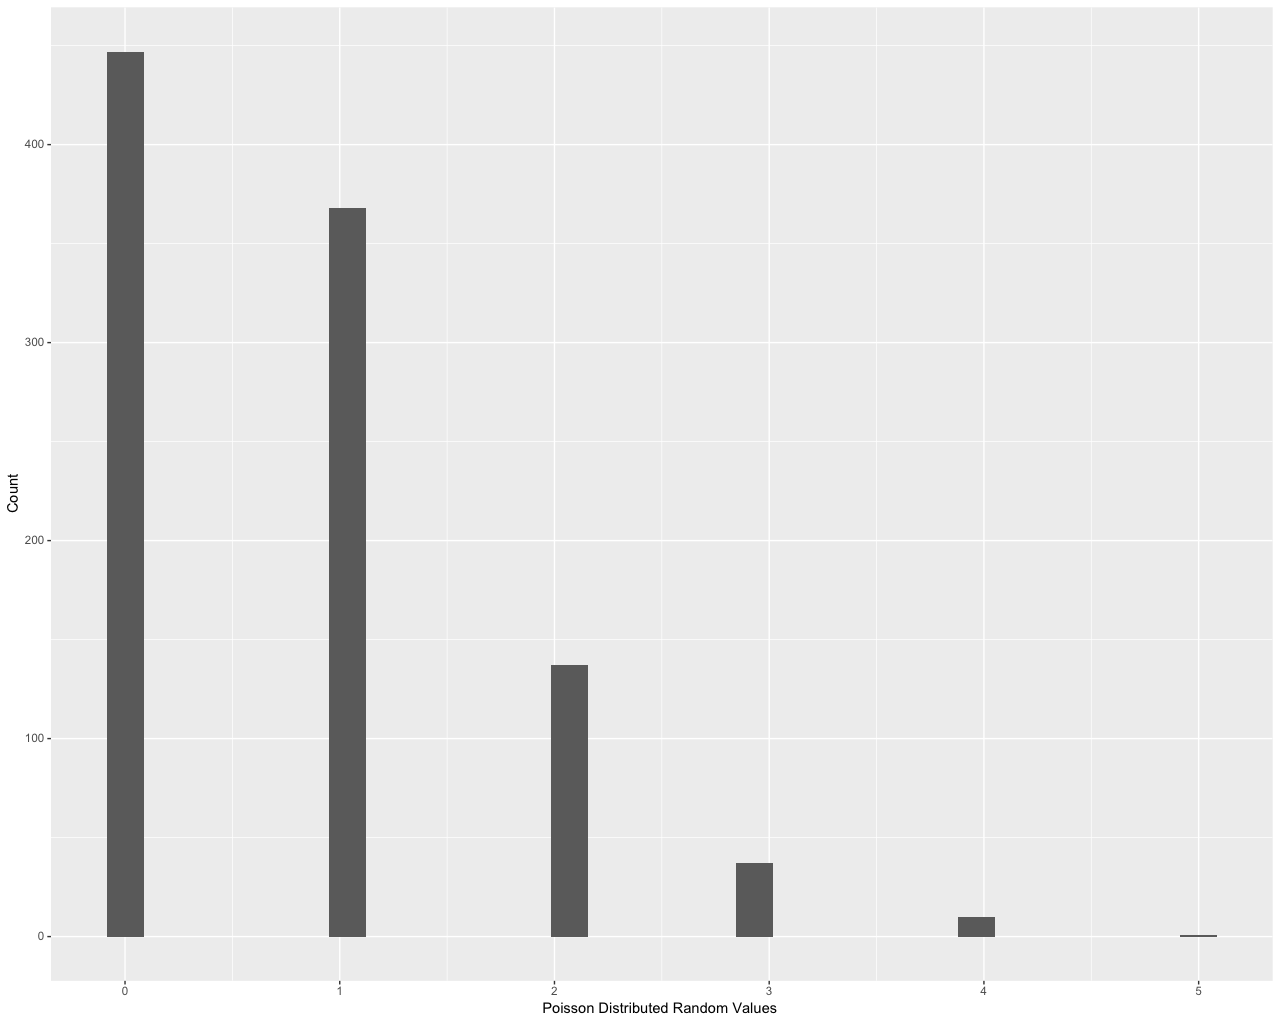
\includegraphics[width=1.0\linewidth]{pic0054}
  \caption{Хистограма на поасоново разпределение}
\label{figure0054}
\end{figure}
\FloatBarrier

С функцията $dpois$ може да се провери плътността за определена стойност (Формула \ref{equation0008}), а с $ppois$ кумулативната стойност. И двете функции могат да се използват с вектор от стойности. 

\subsection{Други разпределения}

Пакетът R предлага богат набор от вероятностни разпределения (Фиг. \ref{figure0055}). Една част от тези разпределения са широко използвани, други не чак толкова.

\begin{figure}[h!]
  \centering
  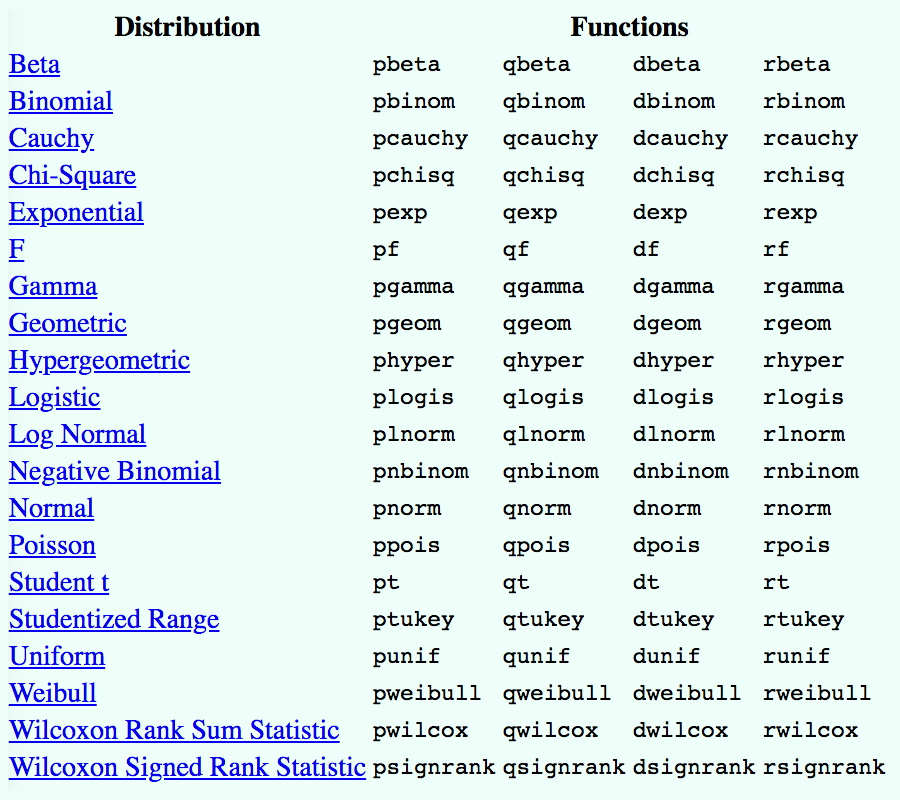
\includegraphics[width=1.0\linewidth]{pic0055}
  \caption{Списък с най-използваните вероятностни разпределения}
\label{figure0055}
\end{figure}
\FloatBarrier

\section*{Заключение}

Визуалното представяне на числените данни повишава степента за възприемане на представяната информация. Колкото по-големи са възможностите на пакетите за визуално представяне, толкова повече възможности биха имали хората работещи с информация и нейното представяне пред широка аудитория. При анализа на случайни величини, визуализацията с хистограма и плътностна функция може да даде най-груба първоначална представа за параметрите на случайната величина. Информация, която може да бъде изключително полезна при избора на по-сложни методи за статистически анализ. От своя страна, визуализацията на случайностите най-удачно се представя, чрез някои от най-използваните вероятностни разпределения. 

